\documentclass[10pt]{article}\usepackage[]{graphicx}\usepackage[]{xcolor}
%% maxwidth is the original width if it is less than linewidth
%% otherwise use linewidth (to make sure the graphics do not exceed the margin)
\makeatletter
\def\maxwidth{ %
  \ifdim\Gin@nat@width>\linewidth
    \linewidth
  \else
    \Gin@nat@width
  \fi
}
\makeatother

\definecolor{fgcolor}{rgb}{0.345, 0.345, 0.345}
\newcommand{\hlnum}[1]{\textcolor[rgb]{0.686,0.059,0.569}{#1}}%
\newcommand{\hlstr}[1]{\textcolor[rgb]{0.192,0.494,0.8}{#1}}%
\newcommand{\hlcom}[1]{\textcolor[rgb]{0.678,0.584,0.686}{\textit{#1}}}%
\newcommand{\hlopt}[1]{\textcolor[rgb]{0,0,0}{#1}}%
\newcommand{\hlstd}[1]{\textcolor[rgb]{0.345,0.345,0.345}{#1}}%
\newcommand{\hlkwa}[1]{\textcolor[rgb]{0.161,0.373,0.58}{\textbf{#1}}}%
\newcommand{\hlkwb}[1]{\textcolor[rgb]{0.69,0.353,0.396}{#1}}%
\newcommand{\hlkwc}[1]{\textcolor[rgb]{0.333,0.667,0.333}{#1}}%
\newcommand{\hlkwd}[1]{\textcolor[rgb]{0.737,0.353,0.396}{\textbf{#1}}}%

\usepackage{framed}
\makeatletter
\newenvironment{kframe}{%
 \def\at@end@of@kframe{}%
 \ifinner\ifhmode%
  \def\at@end@of@kframe{\end{minipage}}%
  \begin{minipage}{\columnwidth}%
 \fi\fi%
 \def\FrameCommand##1{\hskip\@totalleftmargin \hskip-\fboxsep
 \colorbox{shadecolor}{##1}\hskip-\fboxsep
     % There is no \\@totalrightmargin, so:
     \hskip-\linewidth \hskip-\@totalleftmargin \hskip\columnwidth}%
 \MakeFramed {\advance\hsize-\width
   \@totalleftmargin\z@ \linewidth\hsize
   \@setminipage}}%
 {\par\unskip\endMakeFramed%
 \at@end@of@kframe}
\makeatother

\definecolor{shadecolor}{rgb}{.97, .97, .97}
\definecolor{messagecolor}{rgb}{0, 0, 0}
\definecolor{warningcolor}{rgb}{1, 0, 1}
\definecolor{errorcolor}{rgb}{1, 0, 0}
\newenvironment{knitrout}{}{} % an empty environment to be redefined in TeX

\usepackage{alltt}

%%%%%%%%%%%%%%%%%%%%%%%%%%%%%%%%%%%%%%%%%%%%%%%%%%%%%%%%%%%%%%%%%%%%%%%%%%%%%%%%
% LaTeX Imports
%%%%%%%%%%%%%%%%%%%%%%%%%%%%%%%%%%%%%%%%%%%%%%%%%%%%%%%%%%%%%%%%%%%%%%%%%%%%%%%%
\usepackage{amsfonts}                                                   % Math fonts
\usepackage{amsmath}                                                    % Math formatting
\usepackage{amssymb}                                                    % Math formatting
\usepackage{amsthm}                                                     % Math Theorems
\usepackage{arydshln}                                                   % Dashed hlines
\usepackage{attachfile}                                                 % AttachFiles
\usepackage{cancel}                                                     % Cancelled math
\usepackage{caption}                                                    % Figure captioning
\usepackage{color}                                                      % Nice Colors
\input{./lib/dragon.inp}                                                % Tikz dragon curve
\usepackage[ampersand]{easylist}                                        % Easy lists
\usepackage{fancyhdr}                                                   % Fancy Header
\usepackage[T1]{fontenc}                                                % Specific font-encoding
%\usepackage[margin=1in, marginparwidth=2cm, marginparsep=2cm]{geometry} % Margins
\usepackage{graphicx}                                                   % Include images
\usepackage{hyperref}                                                   % Referencing
\usepackage[none]{hyphenat}                                             % Don't allow hyphenation
\usepackage{lipsum}                                                     % Lorem Ipsum Dummy Text
\usepackage{listings}                                                   % Code display
\usepackage{marginnote}                                                 % Notes in the margin
\usepackage{microtype}                                                  % Niceness
\usepackage{lib/minted}                                                 % Code display
\usepackage{multirow}                                                   % Multirow tables
\usepackage{pdfpages}                                                   % Include pdfs
\usepackage{pgfplots}                                                   % Create Pictures
\usepackage{rotating}                                                   % Figure rotation
\usepackage{setspace}                                                   % Allow double spacing
\usepackage{subcaption}                                                 % Figure captioning
\usepackage{tikz}                                                       % Create Pictures
\usepackage{tocloft}                                                    % List of Equations
%%%%%%%%%%%%%%%%%%%%%%%%%%%%%%%%%%%%%%%%%%%%%%%%%%%%%%%%%%%%%%%%%%%%%%%%%%%%%%%%
% Package Setup
%%%%%%%%%%%%%%%%%%%%%%%%%%%%%%%%%%%%%%%%%%%%%%%%%%%%%%%%%%%%%%%%%%%%%%%%%%%%%%%%
\hypersetup{%                                                           % Setup linking
    colorlinks=true,
    linkcolor=black,
    citecolor=black,
    filecolor=black,
    urlcolor=black,
}
\RequirePackage[l2tabu, orthodox]{nag}                                  % Nag about bad syntax
\renewcommand*\thesection{\arabic{section} }                             % Reset numbering
\renewcommand{\theFancyVerbLine}{ {\arabic{FancyVerbLine} } }              % Needed for code display
\renewcommand{\footrulewidth}{0.4pt}                                    % Footer hline
\setcounter{secnumdepth}{3}                                             % Include subsubsections in numbering
\setcounter{tocdepth}{3}                                                % Include subsubsections in toc
%%%%%%%%%%%%%%%%%%%%%%%%%%%%%%%%%%%%%%%%%%%%%%%%%%%%%%%%%%%%%%%%%%%%%%%%%%%%%%%%
% Custom commands
%%%%%%%%%%%%%%%%%%%%%%%%%%%%%%%%%%%%%%%%%%%%%%%%%%%%%%%%%%%%%%%%%%%%%%%%%%%%%%%%
\newcommand{\nvec}[1]{\left\langle #1 \right\rangle}                    %  Easy to use vector
\newcommand{\ma}[0]{\mathbf{A} }                                         %  Easy to use vector
\newcommand{\mb}[0]{\mathbf{B} }                                         %  Easy to use vector
\newcommand{\abs}[1]{\left\lvert #1 \right\rvert}                       %  Easy to use abs
\newcommand{\pren}[1]{\left( #1 \right)}                                %  Big parens
\let\oldvec\vec
\renewcommand{\vec}[1]{\oldvec{\mathbf{#1} } }                            %  Vector Styling
\newtheorem{thm}{Theorem}                                               %  Define the theorem name
\newtheorem{definition}{Definition}                                     %  Define the definition name
\definecolor{bg}{rgb}{0.95,0.95,0.95}
\newcommand{\java}[4]{\vspace{10pt}\inputminted[firstline=#2,
                                 lastline=#3,
                                 firstnumber=#2,
                                 gobble=#4,
                                 frame=single,
                                 label=#1,
                                 bgcolor=bg,
                                 linenos]{java}{#1} }
\newcommand{\python}[4]{\vspace{10pt}\inputminted[firstline=#2,
                                 lastline=#3,
                                 firstnumber=#2,
                                 gobble=#4,
                                 frame=single,
                                 label=#1,
                                 bgcolor=bg,
                                 linenos]{python}{#1} }
\newcommand{\js}[4]{\vspace{10pt}\inputminted[firstline=#2,
                                 lastline=#3,
                                 firstnumber=#2,
                                 gobble=#4,
                                 frame=single,
                                 label=#1,
                                 bgcolor=bg,
                                 linenos]{js}{#1} }
%%%%%%%%%%%%%%%%%%%%%%%%%%%%%%%%%%%%%%%%%%%%%%%%%%%%%%%%%%%%%%%%%%%%%%%%%%%%%%%%
% Beginning of document items - headers, title, toc, etc...
%%%%%%%%%%%%%%%%%%%%%%%%%%%%%%%%%%%%%%%%%%%%%%%%%%%%%%%%%%%%%%%%%%%%%%%%%%%%%%%%
\pagestyle{fancy}                                                       %  Establishes that the headers will be defined
\fancyhead[LE,LO]{Computer Systems Notes}                                  %  Adds header to left
\fancyhead[RE,RO]{Zoe Farmer}                                       %  Adds header to right
\cfoot{ \thepage }
\lfoot{CSCI 2400}
\rfoot{Han}
\title{Computer Systems Notes}
\author{Zoe Farmer}

    \definecolor{orange}{cmyk}{0,0.4,0.8,0.2}
    \definecolor{darkorange}{rgb}{.71,0.21,0.01}
    \definecolor{darkgreen}{rgb}{.12,.54,.11}
    \definecolor{myteal}{rgb}{.26, .44, .56}
    \definecolor{gray}{gray}{0.45}
    \definecolor{lightgray}{gray}{.95}
    \definecolor{mediumgray}{gray}{.8}
    \definecolor{inputbackground}{rgb}{.95, .95, .85}
    \definecolor{outputbackground}{rgb}{.95, .95, .95}
    \definecolor{traceback}{rgb}{1, .95, .95}
    % ansi colors
    \definecolor{red}{rgb}{.6,0,0}
    \definecolor{green}{rgb}{0,.65,0}
    \definecolor{brown}{rgb}{0.6,0.6,0}
    \definecolor{blue}{rgb}{0,.145,.698}
    \definecolor{purple}{rgb}{.698,.145,.698}
    \definecolor{cyan}{rgb}{0,.698,.698}
    \definecolor{lightgray}{gray}{0.5}
    
    % bright ansi colors
    \definecolor{darkgray}{gray}{0.25}
    \definecolor{lightred}{rgb}{1.0,0.39,0.28}
    \definecolor{lightgreen}{rgb}{0.48,0.99,0.0}
    \definecolor{lightblue}{rgb}{0.53,0.81,0.92}
    \definecolor{lightpurple}{rgb}{0.87,0.63,0.87}
    \definecolor{lightcyan}{rgb}{0.5,1.0,0.83}
    
    % commands and environments needed by pandoc snippets
    % extracted from the output of `pandoc -s`
    \DefineVerbatimEnvironment{Highlighting}{Verbatim}{commandchars=\\\{\}}
    % Add ',fontsize=\small' for more characters per line
    \newenvironment{Shaded}{}{}
    \newcommand{\KeywordTok}[1]{\textcolor[rgb]{0.00,0.44,0.13}{\textbf{{#1}}}}
    \newcommand{\DataTypeTok}[1]{\textcolor[rgb]{0.56,0.13,0.00}{{#1}}}
    \newcommand{\DecValTok}[1]{\textcolor[rgb]{0.25,0.63,0.44}{{#1}}}
    \newcommand{\BaseNTok}[1]{\textcolor[rgb]{0.25,0.63,0.44}{{#1}}}
    \newcommand{\FloatTok}[1]{\textcolor[rgb]{0.25,0.63,0.44}{{#1}}}
    \newcommand{\CharTok}[1]{\textcolor[rgb]{0.25,0.44,0.63}{{#1}}}
    \newcommand{\StringTok}[1]{\textcolor[rgb]{0.25,0.44,0.63}{{#1}}}
    \newcommand{\CommentTok}[1]{\textcolor[rgb]{0.38,0.63,0.69}{\textit{{#1}}}}
    \newcommand{\OtherTok}[1]{\textcolor[rgb]{0.00,0.44,0.13}{{#1}}}
    \newcommand{\AlertTok}[1]{\textcolor[rgb]{1.00,0.00,0.00}{\textbf{{#1}}}}
    \newcommand{\FunctionTok}[1]{\textcolor[rgb]{0.02,0.16,0.49}{{#1}}}
    \newcommand{\RegionMarkerTok}[1]{{#1}}
    \newcommand{\ErrorTok}[1]{\textcolor[rgb]{1.00,0.00,0.00}{\textbf{{#1}}}}
    \newcommand{\NormalTok}[1]{{#1}}
    
    % Define a nice break command that doesn't care if a line doesn't already
    % exist.
    \def\br{\hspace*{\fill} \\* }

%%%%%%%%%%%%%%%%%%%%%%%%%%%%%%%%%%%%%%%%%%%%%%%%%%%%%%%%%%%%%%%%%%%%%%%%%%%%%%%%
% Beginning of document items - headers, title, toc, etc...
%%%%%%%%%%%%%%%%%%%%%%%%%%%%%%%%%%%%%%%%%%%%%%%%%%%%%%%%%%%%%%%%%%%%%%%%%%%%%%%%
\pagestyle{fancy}                                                       %  Establishes that the headers will be defined
\fancyhead[LE,LO]{Takehome Final}                                  %  Adds header to left
\fancyhead[RE,RO]{Zoe Farmer}                                       %  Adds header to right
%\cfoot{\mlptikz[size=0.25in, text=on, textposx=0, textposy=0, textvalue=\thepage, textscale=0.75in]{applejack}}
\lfoot{APPM 4570}
\rfoot{Hagar}
\title{Takehome Final}
\author{Zoe Farmer}
%%%%%%%%%%%%%%%%%%%%%%%%%%%%%%%%%%%%%%%%%%%%%%%%%%%%%%%%%%%%%%%%%%%%%%%%%%%%%%%%
% Beginning of document items - headers, title, toc, etc...
%%%%%%%%%%%%%%%%%%%%%%%%%%%%%%%%%%%%%%%%%%%%%%%%%%%%%%%%%%%%%%%%%%%%%%%%%%%%%%%%
\IfFileExists{upquote.sty}{\usepackage{upquote}}{}
\begin{document}

\maketitle




It is January of 1963, and President Kennedy has hired you as the Chief Statistician for the White House.  Your first
task is to analyze and report state expenditures across the country. You feel ready for the challenge, since you studied
so hard in your statistical methods class. On day one, JFK hands you an important data set that contains information on
the 48 states in the contiguous U.S.\ describing per capita state and local public expenditures associated with state
demographic and economic characteristics in 1960.\newline

\noindent You are told that you need to quantify how per capita state and local expenditures can be explained and
predicted by:

\begin{easylist}[itemize]
    @ The economic ability index
    @ The percentage of the population living in a metropolitan area
    @ The percentage change in the population between 1950 and 1960
    @ The percentage of the population aged 5-19 years
    @ The percentage of the population over 65 years old
    @ Whether the state is located in the western part of the United States or not
\end{easylist}

\vspace{0.5cm}

\noindent The variables available in the data set are labeled as follows:

\begin{easylist}[enumerate]
    @ EX: Per capita state and local public expenditures (\$)
    @ ECAB: Economic ability index, in which income, retail sales, and the value of output (manufactures, mineral, and
    agricultural) per capita are equally weighted
    @ MET: Percentage of population living in standard metropolitan areas
    @ GROW: Percent change in population, 1950-1960
    @ YOUNG: Percent of population aged 5-19 years
    @ OLD: Percent of population over 65 years of age
    @ WEST: Western state (1) or not (0)
\end{easylist}

\vspace{0.5cm}

\noindent Keep in mind that the president does not know how to interpret linear model output, and he wants answers in
terms of things that are easily read and understood. Therefore, when analyzing your models, be sure your answers are
friendly for a general audience, but include enough technical information that your statistics professor believes you
know what you're talking about.

\newpage

\section*{Preliminary Setup}

Note, see the attached iPython notebook for complete dynamic codebase.\footnote{Available
    \href{http://nbviewer.ipython.org/gist/anonymous/b97c33b931e25a43bccb}{at this link: http://nbviewer.ipython.org/gist/anonymous/b97c33b931e25a43bccb}.}

    \begin{Verbatim}[commandchars=\\\{\}]
\PY{o}{\PYZpc{}}\PY{k}{pylab} \PY{n}{inline}
\PY{o}{\PYZpc{}}\PY{k}{load\PYZus{}ext} \PY{n}{rmagic}

\PY{k+kn}{from} \PY{n+nn}{IPython.display} \PY{k+kn}{import} \PY{n}{display}\PY{p}{,} \PY{n}{Math}\PY{p}{,} \PY{n}{Latex}

\PY{n}{matplotlib}\PY{o}{.}\PY{n}{rcParams}\PY{p}{[}\PY{l+s}{\PYZsq{}}\PY{l+s}{figure.figsize}\PY{l+s}{\PYZsq{}}\PY{p}{]} \PY{o}{=} \PY{p}{(}\PY{l+m+mi}{8}\PY{p}{,}\PY{l+m+mi}{8}\PY{p}{)}
\PY{n}{rcParams}\PY{p}{[}\PY{l+s}{\PYZsq{}}\PY{l+s}{savefig.dpi}\PY{l+s}{\PYZsq{}}\PY{p}{]} \PY{o}{=} \PY{l+m+mi}{200}

\PY{k+kn}{import} \PY{n+nn}{pandas} \PY{k+kn}{as} \PY{n+nn}{pd}
\PY{k+kn}{import} \PY{n+nn}{numpy} \PY{k+kn}{as} \PY{n+nn}{np}
\PY{k+kn}{import} \PY{n+nn}{scipy.stats} \PY{k+kn}{as} \PY{n+nn}{stats}
\PY{k+kn}{import} \PY{n+nn}{statsmodels.formula.api} \PY{k+kn}{as} \PY{n+nn}{sm}
\PY{k+kn}{import} \PY{n+nn}{matplotlib} \PY{k+kn}{as} \PY{n+nn}{mp}
\PY{k+kn}{import} \PY{n+nn}{matplotlib.pyplot} \PY{k+kn}{as} \PY{n+nn}{plt}
\PY{k+kn}{import} \PY{n+nn}{pandas.tools.plotting} \PY{k+kn}{as} \PY{n+nn}{pp}
\PY{k+kn}{import} \PY{n+nn}{sklearn} \PY{k+kn}{as} \PY{n+nn}{sk}

\PY{n}{data} \PY{o}{=} \PY{n}{pd}\PY{o}{.}\PY{n}{read\PYZus{}csv}\PY{p}{(}\PY{l+s}{\PYZsq{}}\PY{l+s}{./stateExpenditures.csv}\PY{l+s}{\PYZsq{}}\PY{p}{)}  \PY{c}{\PYZsh{} Import our data}

\PY{n}{data}\PY{p}{[}\PY{l+s}{\PYZsq{}}\PY{l+s}{ECAB}\PY{l+s}{\PYZsq{}}\PY{p}{]} \PY{o}{=} \PY{n}{data}\PY{p}{[}\PY{l+s}{\PYZsq{}}\PY{l+s}{ECAB}\PY{l+s}{\PYZsq{}}\PY{p}{]} \PY{o}{\PYZhy{}} \PY{n+nb}{min}\PY{p}{(}\PY{n}{data}\PY{p}{[}\PY{l+s}{\PYZsq{}}\PY{l+s}{ECAB}\PY{l+s}{\PYZsq{}}\PY{p}{]}\PY{p}{)}     \PY{c}{\PYZsh{} Standardize Range}
\PY{n}{data}\PY{p}{[}\PY{l+s}{\PYZsq{}}\PY{l+s}{YOUNG}\PY{l+s}{\PYZsq{}}\PY{p}{]} \PY{o}{=} \PY{n}{data}\PY{p}{[}\PY{l+s}{\PYZsq{}}\PY{l+s}{YOUNG}\PY{l+s}{\PYZsq{}}\PY{p}{]} \PY{o}{\PYZhy{}} \PY{n+nb}{min}\PY{p}{(}\PY{n}{data}\PY{p}{[}\PY{l+s}{\PYZsq{}}\PY{l+s}{YOUNG}\PY{l+s}{\PYZsq{}}\PY{p}{]}\PY{p}{)}  \PY{c}{\PYZsh{} Standardize Range}
\PY{n}{data}\PY{p}{[}\PY{l+s}{\PYZsq{}}\PY{l+s}{OLD}\PY{l+s}{\PYZsq{}}\PY{p}{]} \PY{o}{=} \PY{n}{data}\PY{p}{[}\PY{l+s}{\PYZsq{}}\PY{l+s}{OLD}\PY{l+s}{\PYZsq{}}\PY{p}{]} \PY{o}{\PYZhy{}} \PY{n+nb}{min}\PY{p}{(}\PY{n}{data}\PY{p}{[}\PY{l+s}{\PYZsq{}}\PY{l+s}{OLD}\PY{l+s}{\PYZsq{}}\PY{p}{]}\PY{p}{)}        \PY{c}{\PYZsh{} Standardize Range}
\PY{n}{data}\PY{p}{[}\PY{l+s}{\PYZsq{}}\PY{l+s}{MET\PYZhy{}unst}\PY{l+s}{\PYZsq{}}\PY{p}{]} \PY{o}{=} \PY{n}{data}\PY{p}{[}\PY{l+s}{\PYZsq{}}\PY{l+s}{MET}\PY{l+s}{\PYZsq{}}\PY{p}{]}     \PY{c}{\PYZsh{} Save MET as unstandardized}
\PY{n}{data}\PY{p}{[}\PY{l+s}{\PYZsq{}}\PY{l+s}{MET}\PY{l+s}{\PYZsq{}}\PY{p}{]} \PY{o}{=} \PY{p}{(}\PY{p}{(}\PY{n}{data}\PY{p}{[}\PY{l+s}{\PYZsq{}}\PY{l+s}{MET}\PY{l+s}{\PYZsq{}}\PY{p}{]} \PY{o}{\PYZhy{}} \PY{n}{data}\PY{p}{[}\PY{l+s}{\PYZsq{}}\PY{l+s}{MET}\PY{l+s}{\PYZsq{}}\PY{p}{]}\PY{o}{.}\PY{n}{mean}\PY{p}{(}\PY{p}{)}\PY{p}{)} \PY{o}{/}
              \PY{n}{np}\PY{o}{.}\PY{n}{sqrt}\PY{p}{(}\PY{n}{data}\PY{p}{[}\PY{l+s}{\PYZsq{}}\PY{l+s}{MET}\PY{l+s}{\PYZsq{}}\PY{p}{]}\PY{o}{.}\PY{n}{cov}\PY{p}{(}\PY{n}{data}\PY{p}{[}\PY{l+s}{\PYZsq{}}\PY{l+s}{MET}\PY{l+s}{\PYZsq{}}\PY{p}{]}\PY{p}{)}\PY{p}{)}\PY{p}{)}  \PY{c}{\PYZsh{} Standardize values}

\PY{n}{data}\PY{o}{.}\PY{n}{describe}\PY{p}{(}\PY{p}{)}
\end{Verbatim}

\newpage
            \begin{Verbatim}[commandchars=\\\{\}]
    EX        ECAB           MET       GROW      YOUNG       OLD  \textbackslash{}
count   48.000000   48.000000  4.800000e+01  48.000000  48.000000  48.00000   
mean   286.645833   39.354167  4.440892e-16  18.729167   4.114583   3.81250   
std     58.794807   22.252831  1.000000e+00  18.874749   2.148526   1.63936   
min    183.000000    0.000000 -1.713839e+00  -7.400000   0.000000   0.00000   
25\%    253.500000   28.000000 -8.192181e-01   6.975000   2.400000   2.55000   
50\%    285.500000   37.900000 -6.960222e-04  14.050000   4.000000   4.05000   
75\%    324.000000   47.700000  8.837161e-01  22.675000   5.625000   5.02500   
max    454.000000  147.600000  1.497144e+00  77.800000   8.900000   6.50000   

          WEST   MET-unst  
count  48.000000  48.000000  
mean    0.500000  46.168750  
std     0.505291  26.938797  
min     0.000000   0.000000  
25\%     0.000000  24.100000  
50\%     0.500000  46.150000  
75\%     1.000000  69.975000  
max     1.000000  86.500000  
          
[8 rows x 8 columns]
\end{Verbatim}
        
\newpage

\section*{Part One}
    \subsection*{Question One}
    \textbf{Make scatter plots of the continuous covariates, both against each other and against the outcome
    (expenditures).  Does the relationship between the independent variables and the dependent variables appear to be
    linear? Do there appear to be independent variables that are collinear?}\newline

    We can use \texttt{pandas} built in \texttt{scatter\_matrix} method to plot all random variables against each other.

    \begin{Verbatim}[commandchars=\\\{\}]
\PY{n}{sc\PYZus{}matrix} \PY{o}{=} \PY{n}{pp}\PY{o}{.}\PY{n}{scatter\PYZus{}matrix}\PY{p}{(}\PY{n}{data}\PY{p}{[}\PY{p}{[}\PY{l+s}{\PYZsq{}}\PY{l+s}{EX}\PY{l+s}{\PYZsq{}}\PY{p}{,} \PY{l+s}{\PYZsq{}}\PY{l+s}{ECAB}\PY{l+s}{\PYZsq{}}\PY{p}{,} \PY{l+s}{\PYZsq{}}\PY{l+s}{MET}\PY{l+s}{\PYZsq{}}\PY{p}{,}
                                 \PY{l+s}{\PYZsq{}}\PY{l+s}{GROW}\PY{l+s}{\PYZsq{}}\PY{p}{,} \PY{l+s}{\PYZsq{}}\PY{l+s}{YOUNG}\PY{l+s}{\PYZsq{}}\PY{p}{,} \PY{l+s}{\PYZsq{}}\PY{l+s}{OLD}\PY{l+s}{\PYZsq{}}\PY{p}{]}\PY{p}{]}\PY{p}{,}
                              \PY{n}{alpha}\PY{o}{=}\PY{l+m+mf}{0.7}\PY{p}{,} \PY{n}{figsize}\PY{o}{=}\PY{p}{(}\PY{l+m+mi}{10}\PY{p}{,}\PY{l+m+mi}{10}\PY{p}{)}\PY{p}{)}
    \end{Verbatim}

    \begin{figure}[H]
        \centering
        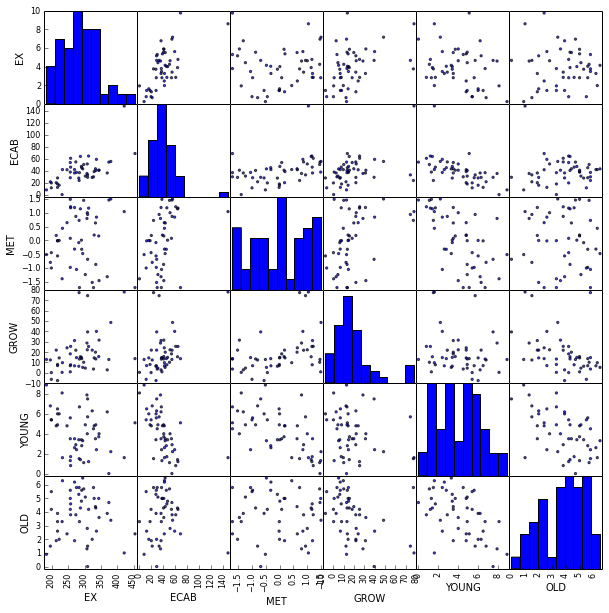
\includegraphics[scale=0.6]{./img/scatter_matrix.png}
        \caption{Scatter Matrix}
        \label{fig:scatter_matrix}
    \end{figure}
    
    We can use \texttt{pandas} built in \texttt{scatter\_matrix} method to plot all random variables against each other.
    When examining this plot we notice several linear relationships immediately, which we can enumerate.

\begin{itemize}
\itemsep1pt\parskip0pt\parsep0pt
\item
  \texttt{EX} vs. \texttt{ECAB}
\item
  \texttt{EX} vs. \texttt{GROW}
\item
  \texttt{EX} vs. \texttt{YOUNG}
\end{itemize}

This is good, as it indicates a good chance that we will be able to create a linear model to predict our dependent
variable, in this case \texttt{EX}.  We also notice some collinearity with our variables, listed below.

\begin{itemize}
\itemsep1pt\parskip0pt\parsep0pt
\item
  \texttt{ECAB} vs. \texttt{MET}
\item
  \texttt{ECAB} vs. \texttt{GROW}
\item
  \texttt{ECAB} vs. \texttt{YOUNG}
\item
  \texttt{ECAB} vs. \texttt{OLD}
\item
  \texttt{MET} vs. \texttt{GROW}
\item
  \texttt{YOUNG} vs. \texttt{OLD}
\end{itemize}

This collinearity is bad, as it will affect any regression we perform.
We will later take steps to remove these collinear variables.

    \subsection*{Question Two}
    \textbf{Fit the following model, converting any variables as you see necessary so that the intercept can be
    interpreted in a meaningful way, and so that variables with a large range are standardized:}

    \begin{equation*}
        \begin{aligned}
            Y_i &=& \beta_0 +
                    \beta_1 \text{ECAB} +
                    \beta_2 \text{MET} +
                    \beta_3 \text{GROW} +\\
                    &&\beta_4 \text{YOUNG} +
                    \beta_5 \text{OLD} +
                    \beta_6 \text{WEST} +
                    \epsilon_i
        \end{aligned}
    \end{equation*}

    \textbf{Write out the estimated regression model. What do you notice about the significance of the parameters in
    this model?}\newline

    We've already standardized the range of several of the variables, as well standardizing \texttt{MET} to the standard
    normal distribution.  Using the Ordinary Least Squares method of linear regression we can create our linear model.

    \begin{Verbatim}[commandchars=\\\{\}]
\PY{c}{\PYZsh{} Multiple linear regression formula}
\PY{n}{multi\PYZus{}regression} \PY{o}{=} \PY{n}{sm}\PY{o}{.}\PY{n}{ols}\PY{p}{(}\PY{n}{formula}\PY{o}{=}\PY{l+s}{\PYZsq{}\PYZsq{}\PYZsq{}}\PY{l+s}{EX \PYZti{} ECAB + MET + GROW +}
\PY{l+s}{                          YOUNG + OLD + WEST}\PY{l+s}{\PYZsq{}\PYZsq{}\PYZsq{}}\PY{p}{,} \PY{n}{data}\PY{o}{=}\PY{n}{data}\PY{p}{)}\PY{o}{.}\PY{n}{fit}\PY{p}{(}\PY{p}{)}
\PY{n}{multi\PYZus{}regression}\PY{o}{.}\PY{n}{summary}\PY{p}{(}\PY{p}{)}
\end{Verbatim}

Resulting in the following output.

            \begin{Verbatim}[commandchars=\\\{\}]
                          OLS Regression Results                            
==============================================================================
Dep. Variable:                     EX   R-squared:                       0.599
Model:                            OLS   Adj. R-squared:                  0.541
Method:                 Least Squares   F-statistic:                     10.22
Date:                Wed, 07 May 2014   Prob (F-statistic):           6.63e-07
Time:                        01:20:52   Log-Likelihood:                -241.20
No. Observations:                  48   AIC:                             496.4
Df Residuals:                      41   BIC:                             509.5
Df Model:                           6                                         
Covariance Type:            nonrobust                                         
==============================================================================
               coef    std err          t      P>|t|      [95.0\% Conf. Int.]
------------------------------------------------------------------------------
Intercept    236.9162     67.850      3.492      0.001        99.890   373.942
ECAB           1.4185      0.430      3.298      0.002         0.550     2.287
MET          -17.7837      9.499     -1.872      0.068       -36.967     1.399
GROW           0.5716      0.425      1.345      0.186        -0.287     1.430
YOUNG         -6.6747      7.481     -0.892      0.377       -21.782     8.433
OLD           -1.8551      7.137     -0.260      0.796       -16.268    12.558
WEST          35.4723     13.771      2.576      0.014         7.661    63.284
==============================================================================
Omnibus:                        0.723   Durbin-Watson:                   2.349
Prob(Omnibus):                  0.697   Jarque-Bera (JB):                0.524
Skew:                           0.253   Prob(JB):                        0.770
Kurtosis:                       2.927   Cond. No.                         602.
==============================================================================
\end{Verbatim}
        
    We immediately notice that the most significant parameter is \texttt{WEST}, followed by \texttt{MET}, followed by
    \texttt{YOUNG}.

    \subsection*{Question Three}
    \textbf{Closely examine the relationship between the percentage of the population living in a metropolitan area and the
    dependent variable. Does this relationship appear to be linear? Add a term to the model you created in part (2) to
    compensate for this non-linearity (justify your thinking), and then write out your estimated model. Does this model
    seem better than the previous model?  Why or why not?}\newline

    Let's examine this plot a little closer by adding a linear and quadratic regression line between \texttt{MET} and
    \texttt{EX} using \texttt{scipy} for our linear regression and \texttt{numpy} for our quadratic regression.

    \begin{Verbatim}[commandchars=\\\{\}]
\PY{c}{\PYZsh{} New two\PYZhy{}var linear regression line}
\PY{n}{ex\PYZus{}met\PYZus{}regression} \PY{o}{=} \PY{n}{sm}\PY{o}{.}\PY{n}{ols}\PY{p}{(}\PY{n}{formula}\PY{o}{=}\PY{l+s}{\PYZsq{}}\PY{l+s}{EX \PYZti{} MET}\PY{l+s}{\PYZsq{}}\PY{p}{,} \PY{n}{data}\PY{o}{=}\PY{n}{data}\PY{p}{)}\PY{o}{.}\PY{n}{fit}\PY{p}{(}\PY{p}{)}\PY{o}{.}\PY{n}{params}
\PY{n}{ex\PYZus{}met\PYZus{}regression}\PY{p}{[}\PY{l+s}{\PYZsq{}}\PY{l+s}{MET2}\PY{l+s}{\PYZsq{}}\PY{p}{]} \PY{o}{=} \PY{l+m+mi}{0}
\PY{c}{\PYZsh{} New two\PYZhy{}var quadratic regression line}
\PY{n}{ex\PYZus{}met\PYZus{}quad}       \PY{o}{=} \PY{n}{np}\PY{o}{.}\PY{n}{polyfit}\PY{p}{(}\PY{n}{data}\PY{p}{[}\PY{l+s}{\PYZsq{}}\PY{l+s}{MET}\PY{l+s}{\PYZsq{}}\PY{p}{]}\PY{p}{,} \PY{n}{data}\PY{p}{[}\PY{l+s}{\PYZsq{}}\PY{l+s}{EX}\PY{l+s}{\PYZsq{}}\PY{p}{]}\PY{p}{,} \PY{l+m+mi}{2}\PY{p}{)}\PY{p}{[}\PY{p}{:}\PY{p}{:}\PY{o}{\PYZhy{}}\PY{l+m+mi}{1}\PY{p}{]}

\PY{n}{pd}\PY{o}{.}\PY{n}{DataFrame}\PY{p}{(}\PY{p}{\PYZob{}}\PY{l+s}{\PYZsq{}}\PY{l+s}{Linear Model}\PY{l+s}{\PYZsq{}}\PY{p}{:}\PY{n}{ex\PYZus{}met\PYZus{}regression}\PY{p}{,}
              \PY{l+s}{\PYZsq{}}\PY{l+s}{Quadratic Model}\PY{l+s}{\PYZsq{}}\PY{p}{:}\PY{n}{ex\PYZus{}met\PYZus{}quad}\PY{p}{\PYZcb{}}\PY{p}{)}
\end{Verbatim}

\begin{Verbatim}[commandchars=\\\{\}]
Linear Model  Quadratic Model
Intercept    286.645833       255.121129
MET            2.659590         7.676721
MET2           0.000000        32.195443

[3 rows x 2 columns]
\end{Verbatim}

    Now we'll plot our two regression lines along with the scatter plot of \texttt{EX \textasciitilde{} MET}.

    \begin{Verbatim}[commandchars=\\\{\}]
\PY{n}{fig}\PY{p}{,} \PY{n}{ax} \PY{o}{=} \PY{n}{plt}\PY{o}{.}\PY{n}{subplots}\PY{p}{(}\PY{p}{)}
\PY{n}{x}       \PY{o}{=} \PY{n}{np}\PY{o}{.}\PY{n}{arange}\PY{p}{(}\PY{o}{\PYZhy{}}\PY{l+m+mi}{2}\PY{p}{,} \PY{l+m+mi}{3}\PY{p}{,} \PY{l+m+mf}{0.01}\PY{p}{)}
\PY{n}{ax}\PY{o}{.}\PY{n}{scatter}\PY{p}{(}\PY{n}{data}\PY{p}{[}\PY{l+s}{\PYZsq{}}\PY{l+s}{MET}\PY{l+s}{\PYZsq{}}\PY{p}{]}\PY{p}{,} \PY{n}{data}\PY{p}{[}\PY{l+s}{\PYZsq{}}\PY{l+s}{EX}\PY{l+s}{\PYZsq{}}\PY{p}{]}\PY{p}{,}
           \PY{n}{label}\PY{o}{=}\PY{l+s}{\PYZsq{}}\PY{l+s}{EX\PYZti{}MET}\PY{l+s}{\PYZsq{}}\PY{p}{)}  \PY{c}{\PYZsh{} EX\PYZti{}MET scatter}
\PY{c}{\PYZsh{} Linear Regresssion Line}
\PY{n}{ax}\PY{o}{.}\PY{n}{plot}\PY{p}{(}\PY{n}{x}\PY{p}{,} \PY{n}{ex\PYZus{}met\PYZus{}regression}\PY{p}{[}\PY{l+m+mi}{0}\PY{p}{]} \PY{o}{+} 
      \PY{n}{ex\PYZus{}met\PYZus{}regression}\PY{p}{[}\PY{l+m+mi}{1}\PY{p}{]} \PY{o}{*} \PY{n}{x}\PY{p}{,}
      \PY{n}{label}\PY{o}{=}\PY{p}{(}\PY{l+s}{r\PYZsq{}}\PY{l+s}{Linear Regression}\PY{l+s}{\PYZsq{}}
             \PY{l+s}{\PYZsq{}}\PY{l+s+se}{\PYZbs{}n}\PY{l+s}{\PYZsq{}}
             \PY{l+s}{r\PYZsq{}}\PY{l+s}{\PYZdl{}}\PY{l+s}{\PYZbs{}}\PY{l+s}{hat\PYZob{}}\PY{l+s}{\PYZbs{}}\PY{l+s}{beta\PYZcb{}\PYZus{}1 }\PY{l+s}{\PYZbs{}}\PY{l+s}{cdot x + }\PY{l+s}{\PYZbs{}}\PY{l+s}{hat\PYZob{}}\PY{l+s}{\PYZbs{}}\PY{l+s}{beta\PYZcb{}\PYZus{}0\PYZdl{}}\PY{l+s}{\PYZsq{}}\PY{p}{)}\PY{p}{)}
\PY{c}{\PYZsh{} Quadratic Regresssion Line}
\PY{n}{ax}\PY{o}{.}\PY{n}{plot}\PY{p}{(}\PY{n}{x}\PY{p}{,} \PY{n}{ex\PYZus{}met\PYZus{}quad}\PY{p}{[}\PY{l+m+mi}{2}\PY{p}{]} \PY{o}{*} \PY{n}{x}\PY{o}{*}\PY{o}{*}\PY{l+m+mi}{2} \PY{o}{+}
      \PY{n}{ex\PYZus{}met\PYZus{}quad}\PY{p}{[}\PY{l+m+mi}{1}\PY{p}{]} \PY{o}{*} \PY{n}{x} \PY{o}{+} \PY{n}{ex\PYZus{}met\PYZus{}quad}\PY{p}{[}\PY{l+m+mi}{0}\PY{p}{]}\PY{p}{,}
      \PY{n}{label}\PY{o}{=}\PY{p}{(}\PY{l+s}{r\PYZsq{}}\PY{l+s}{Quadratic Regression}\PY{l+s}{\PYZsq{}}
             \PY{l+s}{\PYZsq{}}\PY{l+s+se}{\PYZbs{}n}\PY{l+s}{\PYZsq{}}
             \PY{l+s}{r\PYZsq{}}\PY{l+s}{\PYZdl{}}\PY{l+s}{\PYZbs{}}\PY{l+s}{hat\PYZob{}}\PY{l+s}{\PYZbs{}}\PY{l+s}{beta\PYZcb{}\PYZus{}2 }\PY{l+s}{\PYZbs{}}\PY{l+s}{cdot x\PYZca{}2 + }\PY{l+s}{\PYZbs{}}\PY{l+s}{hat\PYZob{}}\PY{l+s}{\PYZbs{}}\PY{l+s}{beta\PYZcb{}\PYZus{}1 }\PY{l+s}{\PYZbs{}}\PY{l+s}{cdot x + }
             \PY{l+s}{\PYZbs{}}\PY{l+s}{hat\PYZob{}}\PY{l+s}{\PYZbs{}}\PY{l+s}{beta\PYZcb{}\PYZus{}0\PYZdl{}}\PY{l+s}{\PYZsq{}}\PY{p}{)}\PY{p}{)}
\PY{n}{handles}\PY{p}{,} \PY{n}{labels} \PY{o}{=} \PY{n}{ax}\PY{o}{.}\PY{n}{get\PYZus{}legend\PYZus{}handles\PYZus{}labels}\PY{p}{(}\PY{p}{)}
\PY{n}{ax}\PY{o}{.}\PY{n}{legend}\PY{p}{(}\PY{n}{handles}\PY{p}{,} \PY{n}{labels}\PY{p}{)}
\PY{n}{ax}\PY{o}{.}\PY{n}{grid}\PY{p}{(}\PY{n+nb+bp}{True}\PY{p}{,} \PY{n}{which}\PY{o}{=}\PY{l+s}{\PYZsq{}}\PY{l+s}{both}\PY{l+s}{\PYZsq{}}\PY{p}{)}
\PY{n}{plt}\PY{o}{.}\PY{n}{xlabel}\PY{p}{(}\PY{l+s}{\PYZsq{}}\PY{l+s}{MET}\PY{l+s}{\PYZsq{}}\PY{p}{)}
\PY{n}{plt}\PY{o}{.}\PY{n}{ylabel}\PY{p}{(}\PY{l+s}{\PYZsq{}}\PY{l+s}{EX}\PY{l+s}{\PYZsq{}}\PY{p}{)}
\PY{n}{plt}\PY{o}{.}\PY{n}{xlim}\PY{p}{(}\PY{p}{(}\PY{o}{\PYZhy{}}\PY{l+m+mi}{2}\PY{p}{,}\PY{l+m+mi}{2}\PY{p}{)}\PY{p}{)}
\PY{n}{plt}\PY{o}{.}\PY{n}{ylim}\PY{p}{(}\PY{p}{(}\PY{l+m+mi}{150}\PY{p}{,} \PY{l+m+mi}{500}\PY{p}{)}\PY{p}{)}
\PY{n}{plt}\PY{o}{.}\PY{n}{show}\PY{p}{(}\PY{p}{)}
\end{Verbatim}

    \begin{figure}[H]
        \centering
        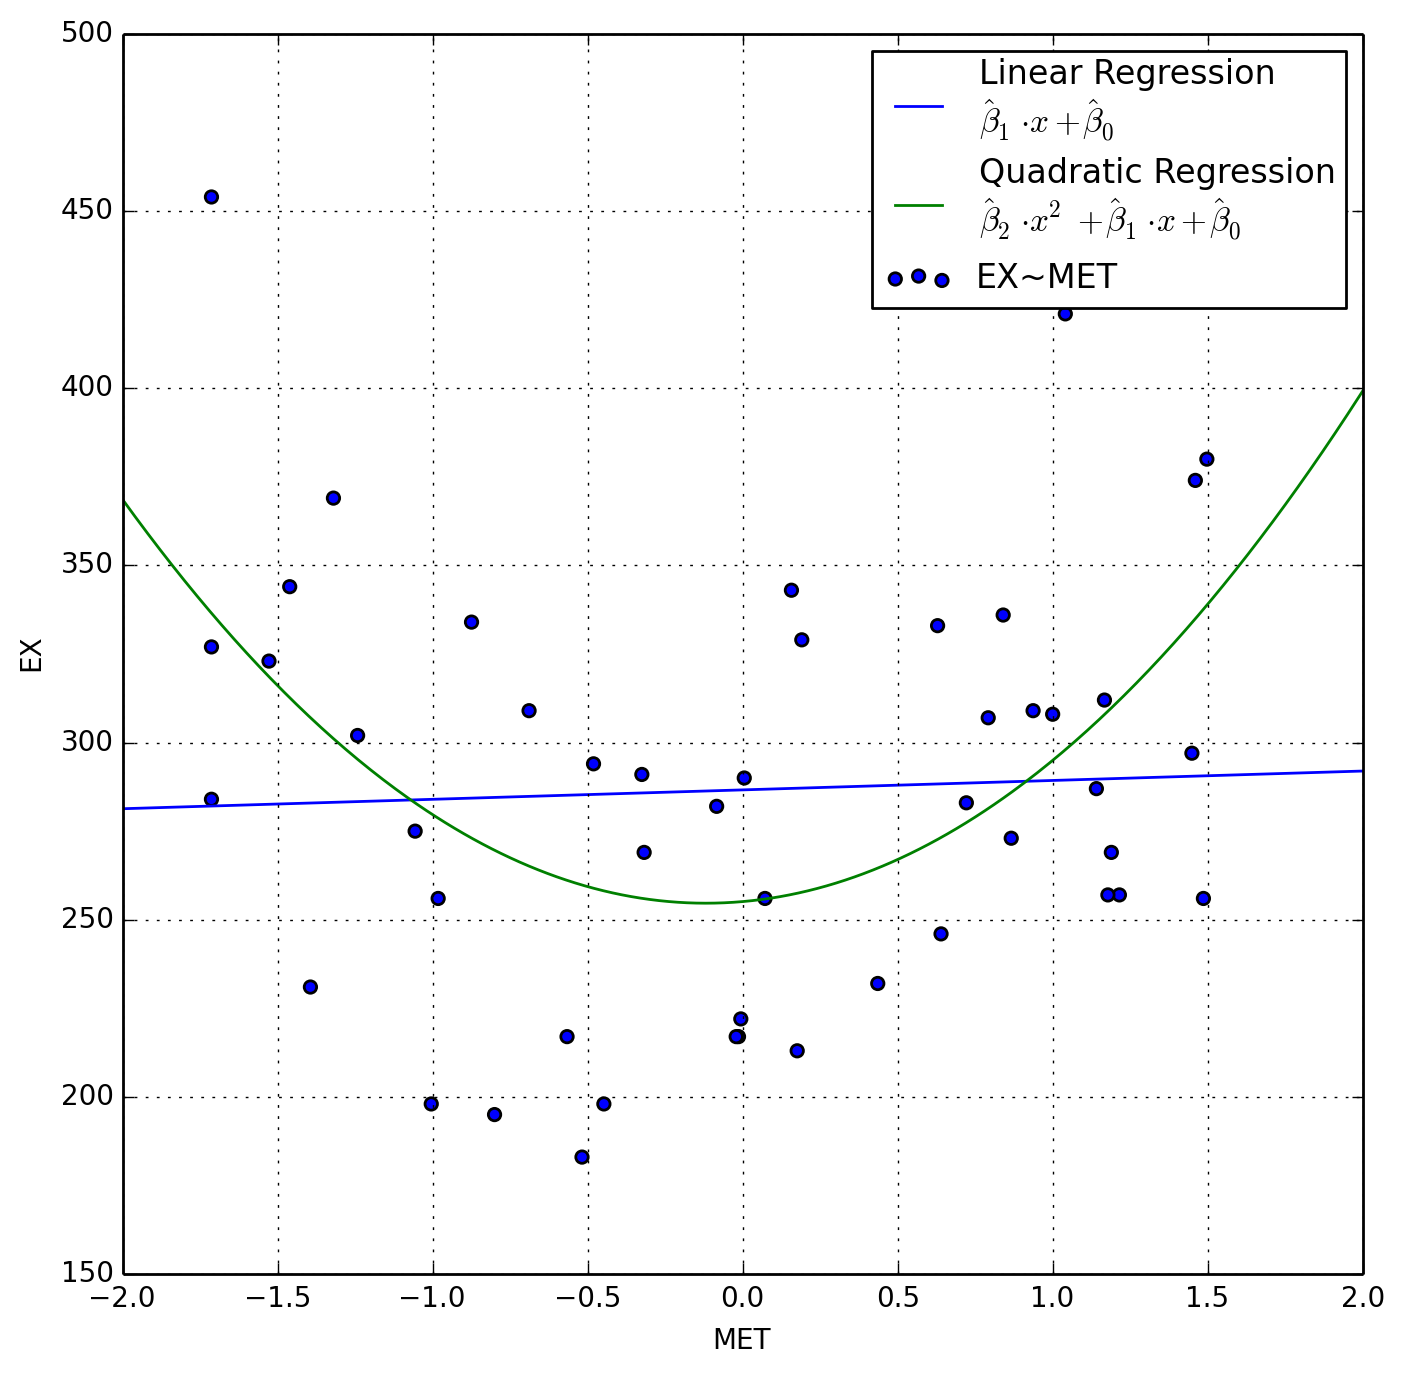
\includegraphics[scale=0.6]{./img/lin_quad.png}
        \caption{Linear/Quadratic Models}
        \label{fig:linquad}
    \end{figure}
    
    We immediately notice that our regression is \emph{not} linear, and in fact appears to be quadratic. When we compare
    our two models, one linear and one quadratic, the quadratic model appears to fit the data much better.

    \begin{equation}
        \begin{aligned}
            f(x) &=& 32.1954 \cdot x^2 + 7.6767 \cdot x + 255.1211& \qquad \to \text{Quadratic}\\
            f(x) &=& 2.6595 \cdot x + 286.6458& \qquad \to \text{Linear}
        \end{aligned}
    \end{equation}

We can add a new column to our data, in this case $\text{MET}^2$, which we'll call \texttt{MET2}. Since we've shown a
quadratic model to fit this particular variable, we can add a squared version of it to our dataset. We can now plot
\texttt{EX\textasciitilde{}MET2} do demonstrate the now linear relationship between the two random variables.

    \begin{Verbatim}[commandchars=\\\{\}]
\PY{c}{\PYZsh{} Add variable to data}
\PY{n}{data}\PY{p}{[}\PY{l+s}{\PYZsq{}}\PY{l+s}{MET2}\PY{l+s}{\PYZsq{}}\PY{p}{]} \PY{o}{=} \PY{n}{pd}\PY{o}{.}\PY{n}{Series}\PY{p}{(}\PY{n}{data}\PY{p}{[}\PY{l+s}{\PYZsq{}}\PY{l+s}{MET}\PY{l+s}{\PYZsq{}}\PY{p}{]}\PY{o}{*}\PY{o}{*}\PY{l+m+mi}{2}\PY{p}{,} \PY{n}{index}\PY{o}{=}\PY{n}{data}\PY{o}{.}\PY{n}{index}\PY{p}{)}

\PY{c}{\PYZsh{} New linear regression}
\PY{n}{ex\PYZus{}met2} \PY{o}{=} \PY{n}{np}\PY{o}{.}\PY{n}{polyfit}\PY{p}{(}\PY{n}{data}\PY{p}{[}\PY{l+s}{\PYZsq{}}\PY{l+s}{MET2}\PY{l+s}{\PYZsq{}}\PY{p}{]}\PY{p}{,} \PY{n}{data}\PY{p}{[}\PY{l+s}{\PYZsq{}}\PY{l+s}{EX}\PY{l+s}{\PYZsq{}}\PY{p}{]}\PY{p}{,} \PY{l+m+mi}{1}\PY{p}{)}

\PY{n}{fig}\PY{p}{,} \PY{n}{ax} \PY{o}{=} \PY{n}{plt}\PY{o}{.}\PY{n}{subplots}\PY{p}{(}\PY{p}{)}
\PY{n}{ax}\PY{o}{.}\PY{n}{scatter}\PY{p}{(}\PY{n}{data}\PY{p}{[}\PY{l+s}{\PYZsq{}}\PY{l+s}{MET2}\PY{l+s}{\PYZsq{}}\PY{p}{]}\PY{p}{,} \PY{n}{data}\PY{p}{[}\PY{l+s}{\PYZsq{}}\PY{l+s}{EX}\PY{l+s}{\PYZsq{}}\PY{p}{]}\PY{p}{,} \PY{n}{label}\PY{o}{=}\PY{l+s}{\PYZsq{}}\PY{l+s}{MET2\PYZti{}EX}\PY{l+s}{\PYZsq{}}\PY{p}{)}
\PY{n}{x} \PY{o}{=} \PY{n}{np}\PY{o}{.}\PY{n}{arange}\PY{p}{(}\PY{l+m+mi}{0}\PY{p}{,} \PY{l+m+mf}{3.5}\PY{p}{)}
\PY{n}{ax}\PY{o}{.}\PY{n}{plot}\PY{p}{(}\PY{n}{x}\PY{p}{,} \PY{n}{ex\PYZus{}met2}\PY{p}{[}\PY{l+m+mi}{0}\PY{p}{]} \PY{o}{*} \PY{n}{x} \PY{o}{+} \PY{n}{ex\PYZus{}met2}\PY{p}{[}\PY{l+m+mi}{1}\PY{p}{]}\PY{p}{,} \PY{n}{label}\PY{o}{=}\PY{l+s}{\PYZsq{}}\PY{l+s}{Linear Model}\PY{l+s}{\PYZsq{}}\PY{p}{)}
\PY{n}{ax}\PY{o}{.}\PY{n}{grid}\PY{p}{(}\PY{n+nb+bp}{True}\PY{p}{,} \PY{n}{which}\PY{o}{=}\PY{l+s}{\PYZsq{}}\PY{l+s}{both}\PY{l+s}{\PYZsq{}}\PY{p}{)}
\PY{n}{ax}\PY{o}{.}\PY{n}{set\PYZus{}xlabel}\PY{p}{(}\PY{l+s}{\PYZsq{}}\PY{l+s}{MET2}\PY{l+s}{\PYZsq{}}\PY{p}{)}
\PY{n}{ax}\PY{o}{.}\PY{n}{set\PYZus{}ylabel}\PY{p}{(}\PY{l+s}{\PYZsq{}}\PY{l+s}{EX}\PY{l+s}{\PYZsq{}}\PY{p}{)}
\PY{n}{handles}\PY{p}{,} \PY{n}{labels} \PY{o}{=} \PY{n}{ax}\PY{o}{.}\PY{n}{get\PYZus{}legend\PYZus{}handles\PYZus{}labels}\PY{p}{(}\PY{p}{)}
\PY{n}{ax}\PY{o}{.}\PY{n}{legend}\PY{p}{(}\PY{n}{handles}\PY{p}{,} \PY{n}{labels}\PY{p}{)}
\PY{n}{plt}\PY{o}{.}\PY{n}{xlim}\PY{p}{(}\PY{p}{(}\PY{l+m+mi}{0}\PY{p}{,} \PY{l+m+mi}{3}\PY{p}{)}\PY{p}{)}
\PY{n}{plt}\PY{o}{.}\PY{n}{show}\PY{p}{(}\PY{p}{)}
\end{Verbatim}

    \begin{figure}[H]
        \centering
        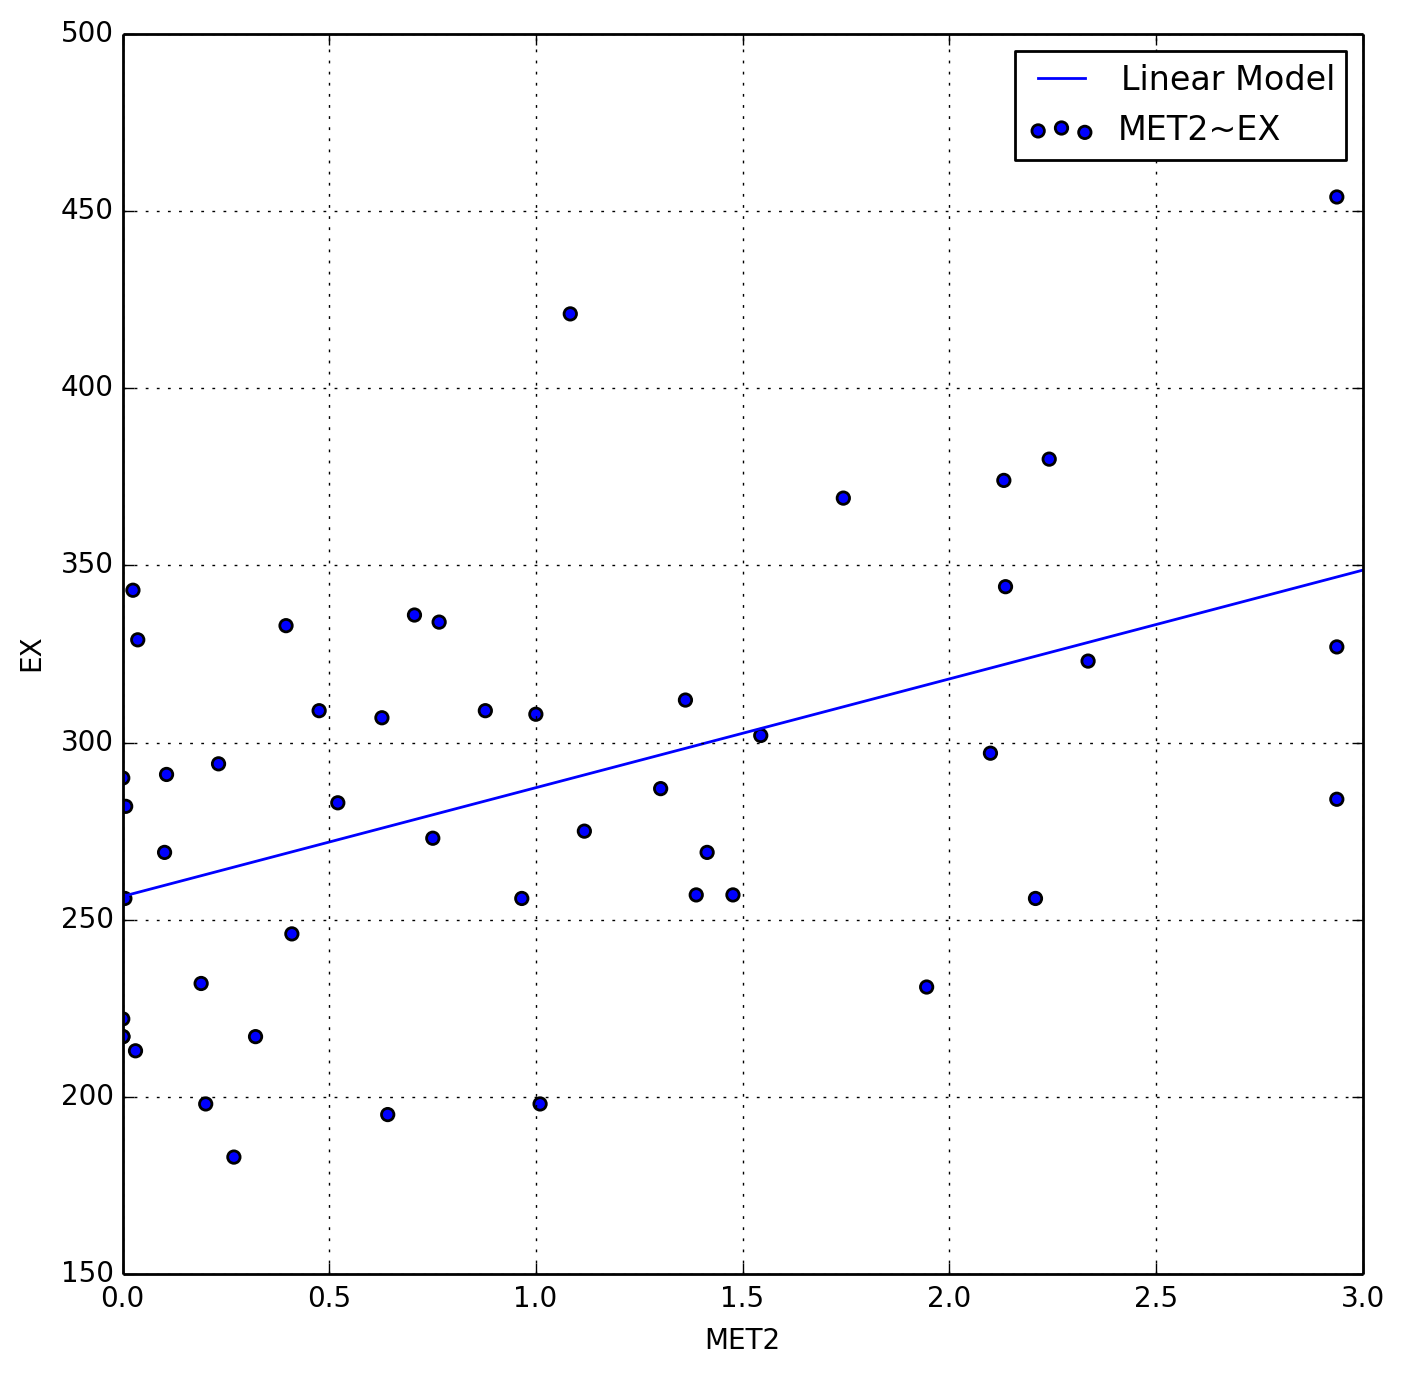
\includegraphics[scale=0.6]{./img/squarefit.png}
        \caption{MET2 Linear Fit}
        \label{fig:met2fit}
    \end{figure}
    
    We also examine the adjusted coefficients of determination for both our
linear and quadratic model which is defined as

\begin{equation}
\bar R^2 = {R^{2}-(1-R^{2}){p \over n-p-1}}
\end{equation}

\begin{Verbatim}[commandchars=\\\{\}]
\PY{o}{\PYZpc{}}\PY{k}{R} \PY{o}{\PYZhy{}}\PY{n}{o} \PY{n}{quadr2} \PY{n}{quadr2} \PY{o}{\PYZlt{}}\PY{o}{\PYZhy{}} \PY{n}{summary}\PY{p}{(}\PY{n}{lm}\PY{p}{(}\PY{n}{EX} \PY{o}{\PYZti{}} \PY{n}{MET} \PY{o}{+} \PY{n}{MET2}\PY{p}{,} \PY{n}{data}\PY{o}{=}\PY{n}{data}\PY{p}{)}\PY{p}{)}\PY{err}{\PYZdl{}}\PY{n}{adj}\PY{o}{.}\PY{n}{r}\PY{o}{.}\PY{n}{squared}
\PY{o}{\PYZpc{}}\PY{k}{R} \PY{o}{\PYZhy{}}\PY{n}{o} \PY{n}{linr2} \PY{n}{linr2} \PY{o}{\PYZlt{}}\PY{o}{\PYZhy{}} \PY{n}{summary}\PY{p}{(}\PY{n}{lm}\PY{p}{(}\PY{n}{EX} \PY{o}{\PYZti{}} \PY{n}{MET}\PY{p}{,} \PY{n}{data}\PY{o}{=}\PY{n}{data}\PY{p}{)}\PY{p}{)}\PY{err}{\PYZdl{}}\PY{n}{adj}\PY{o}{.}\PY{n}{r}\PY{o}{.}\PY{n}{squared}

\PY{k}{print}\PY{p}{(}\PY{l+s}{\PYZsq{}}\PY{l+s}{Quadratic R2:  }\PY{l+s}{\PYZsq{}}\PY{p}{,} \PY{n}{quadr2}\PY{p}{[}\PY{l+m+mi}{0}\PY{p}{]}\PY{p}{)}
\PY{k}{print}\PY{p}{(}\PY{l+s}{\PYZsq{}}\PY{l+s}{Linear R2:    }\PY{l+s}{\PYZsq{}}\PY{p}{,} \PY{n}{linr2}\PY{p}{[}\PY{l+m+mi}{0}\PY{p}{]}\PY{p}{)}
\end{Verbatim}

    \begin{Verbatim}[commandchars=\\\{\}]
Quadratic R2:   0.198787097218
Linear R2:     -0.0196484323278
    \end{Verbatim}

    Note, our quadratic model is an order of magnitude better at explaining the relationship between the two variables.
    This essentially boils down to the fact that we \emph{should} favor the quadratic model over the linear one in the
    future.

    \subsection*{Question Four}
    \textbf{Self-performed model selection: starting with the full model created in part (3): remove the predictor with
    the highest p-value, and re-calculate the model without that predictor. Continue this process until there are no
    predictors left with p-values greater than 0.05. Write out your final estimated model. Do you think that this model
    is better than the full model? Why or why not?}\newline

    We've already calculated our p-values for our multiple regression, so we can examine values that exceed 0.05.

    \begin{Verbatim}[commandchars=\\\{\}]
 \PY{n}{sm}\PY{o}{.}\PY{n}{ols}\PY{p}{(}\PY{n}{formula}\PY{o}{=}\PY{p}{(}\PY{l+s}{\PYZsq{}}\PY{l+s}{EX \PYZti{} ECAB + MET + MET2 + GROW + YOUNG +}\PY{l+s}{\PYZsq{}}
                          \PY{l+s}{\PYZsq{}}\PY{l+s}{OLD + WEST}\PY{l+s}{\PYZsq{}}\PY{p}{)}\PY{p}{,} \PY{n}{data}\PY{o}{=}\PY{n}{data}\PY{p}{)}\PY{o}{.}\PY{n}{fit}\PY{p}{(}\PY{p}{)}\PY{o}{.}\PY{n}{pvalues}
\end{Verbatim}

            \begin{Verbatim}[commandchars=\\\{\}]
Intercept    0.015912
ECAB         0.000749
MET          0.586313
MET2         0.001332
GROW         0.074371
YOUNG        0.931018
OLD          0.534383
WEST         0.008192
dtype: float64
\end{Verbatim}
        
    We can now remove the fields with greater p-values one at a time, examining the p-values as we go. First is
    \texttt{YOUNG}.

    \begin{Verbatim}[commandchars=\\\{\}]
\PY{n}{sm}\PY{o}{.}\PY{n}{ols}\PY{p}{(}\PY{n}{formula}\PY{o}{=}\PY{l+s}{\PYZsq{}\PYZsq{}\PYZsq{}}\PY{l+s}{EX \PYZti{} ECAB + MET + MET2 + GROW + OLD + WEST}\PY{l+s}{\PYZsq{}\PYZsq{}\PYZsq{}}\PY{p}{,}
        \PY{n}{data}\PY{o}{=}\PY{n}{data}\PY{p}{)}\PY{o}{.}\PY{n}{fit}\PY{p}{(}\PY{p}{)}\PY{o}{.}\PY{n}{pvalues}
\end{Verbatim}

            \begin{Verbatim}[commandchars=\\\{\}]
Intercept    6.434445e-11
ECAB         2.144302e-05
MET          4.074601e-01
MET2         7.624931e-04
GROW         6.430896e-02
OLD          3.042440e-01
WEST         3.719836e-03
dtype: float64
\end{Verbatim}
        
    Next is \texttt{MET}

    \begin{Verbatim}[commandchars=\\\{\}]
\PY{n}{sm}\PY{o}{.}\PY{n}{ols}\PY{p}{(}\PY{n}{formula}\PY{o}{=}\PY{l+s}{\PYZsq{}\PYZsq{}\PYZsq{}}\PY{l+s}{EX \PYZti{} ECAB + MET2 + GROW + OLD + WEST}\PY{l+s}{\PYZsq{}\PYZsq{}\PYZsq{}}\PY{p}{,}
         \PY{n}{data}\PY{o}{=}\PY{n}{data}\PY{p}{)}\PY{o}{.}\PY{n}{fit}\PY{p}{(}\PY{p}{)}\PY{o}{.}\PY{n}{pvalues}
\end{Verbatim}

            \begin{Verbatim}[commandchars=\\\{\}]
Intercept    1.953933e-11
ECAB         1.934543e-05
MET2         2.193928e-04
GROW         9.082126e-02
OLD          3.421252e-01
WEST         4.504071e-04
dtype: float64
\end{Verbatim}
        
    Next is \texttt{OLD}

    \begin{Verbatim}[commandchars=\\\{\}]
\PY{n}{sm}\PY{o}{.}\PY{n}{ols}\PY{p}{(}\PY{n}{formula}\PY{o}{=}\PY{l+s}{\PYZsq{}\PYZsq{}\PYZsq{}}\PY{l+s}{EX \PYZti{} ECAB + MET2 + GROW + WEST}\PY{l+s}{\PYZsq{}\PYZsq{}\PYZsq{}}\PY{p}{,}
        \PY{n}{data}\PY{o}{=}\PY{n}{data}\PY{p}{)}\PY{o}{.}\PY{n}{fit}\PY{p}{(}\PY{p}{)}\PY{o}{.}\PY{n}{pvalues}
\end{Verbatim}

            \begin{Verbatim}[commandchars=\\\{\}]
Intercept    4.954987e-19
ECAB         7.617470e-06
MET2         2.400175e-04
GROW         1.523282e-01
WEST         4.430367e-04
dtype: float64
\end{Verbatim}
        
    Next is \texttt{Grow}

    \begin{Verbatim}[commandchars=\\\{\}]
\PY{n}{purged\PYZus{}multi\PYZus{}regression} \PY{o}{=} \PY{n}{sm}\PY{o}{.}\PY{n}{ols}\PY{p}{(}\PY{n}{formula}\PY{o}{=}\PY{l+s}{\PYZsq{}\PYZsq{}\PYZsq{}}\PY{l+s}{EX \PYZti{} ECAB + MET2 + WEST}\PY{l+s}{\PYZsq{}\PYZsq{}\PYZsq{}}\PY{p}{,}
        \PY{n}{data}\PY{o}{=}\PY{n}{data}\PY{p}{)}\PY{o}{.}\PY{n}{fit}\PY{p}{(}\PY{p}{)}
\PY{n}{purged\PYZus{}multi\PYZus{}regression}\PY{o}{.}\PY{n}{summary}\PY{p}{(}\PY{p}{)}
\end{Verbatim}

\begin{Verbatim}[commandchars=\\\{\}]
                          OLS Regression Results                            
==============================================================================
Dep. Variable:                     EX   R-squared:                       0.663
Model:                            OLS   Adj. R-squared:                  0.640
Method:                 Least Squares   F-statistic:                     28.88
Date:                Wed, 07 May 2014   Prob (F-statistic):           1.77e-10
Time:                        01:21:20   Log-Likelihood:                -237.04
No. Observations:                  48   AIC:                             482.1
Df Residuals:                      44   BIC:                             489.6
Df Model:                           3                                         
Covariance Type:            nonrobust                                         
==============================================================================
               coef    std err          t      P>|t|      [95.0\% Conf. Int.]
------------------------------------------------------------------------------
Intercept    184.9759     12.072     15.323      0.000       160.646   209.306
ECAB           1.5199      0.236      6.444      0.000         1.045     1.995
MET2          22.5489      5.888      3.829      0.000        10.682    34.416
WEST          39.5505     10.191      3.881      0.000        19.012    60.089
==============================================================================
Omnibus:                        1.897   Durbin-Watson:                   2.613
Prob(Omnibus):                  0.387   Jarque-Bera (JB):                1.261
Skew:                          -0.095   Prob(JB):                        0.532
Kurtosis:                       2.229   Cond. No.                         119.
==============================================================================
\end{Verbatim}
        
    And we finally obtain our model with large p-values removed containing
\emph{only} \texttt{ECAB}, \texttt{MET2}, and \texttt{WEST}. We can
create another scatter plot to show only our selected variables.

    \begin{Verbatim}[commandchars=\\\{\}]
\PY{n}{sc\PYZus{}matrix} \PY{o}{=} \PY{n}{pp}\PY{o}{.}\PY{n}{scatter\PYZus{}matrix}\PY{p}{(}\PY{n}{data}\PY{p}{[}\PY{p}{[}\PY{l+s}{\PYZsq{}}\PY{l+s}{EX}\PY{l+s}{\PYZsq{}}\PY{p}{,} \PY{l+s}{\PYZsq{}}\PY{l+s}{ECAB}\PY{l+s}{\PYZsq{}}\PY{p}{,} \PY{l+s}{\PYZsq{}}\PY{l+s}{MET2}\PY{l+s}{\PYZsq{}}\PY{p}{,} \PY{l+s}{\PYZsq{}}\PY{l+s}{WEST}\PY{l+s}{\PYZsq{}}\PY{p}{]}\PY{p}{]}\PY{p}{,}
                                     \PY{n}{alpha}\PY{o}{=}\PY{l+m+mf}{0.7}\PY{p}{)}
\end{Verbatim}

    \begin{figure}[H]
        \centering
        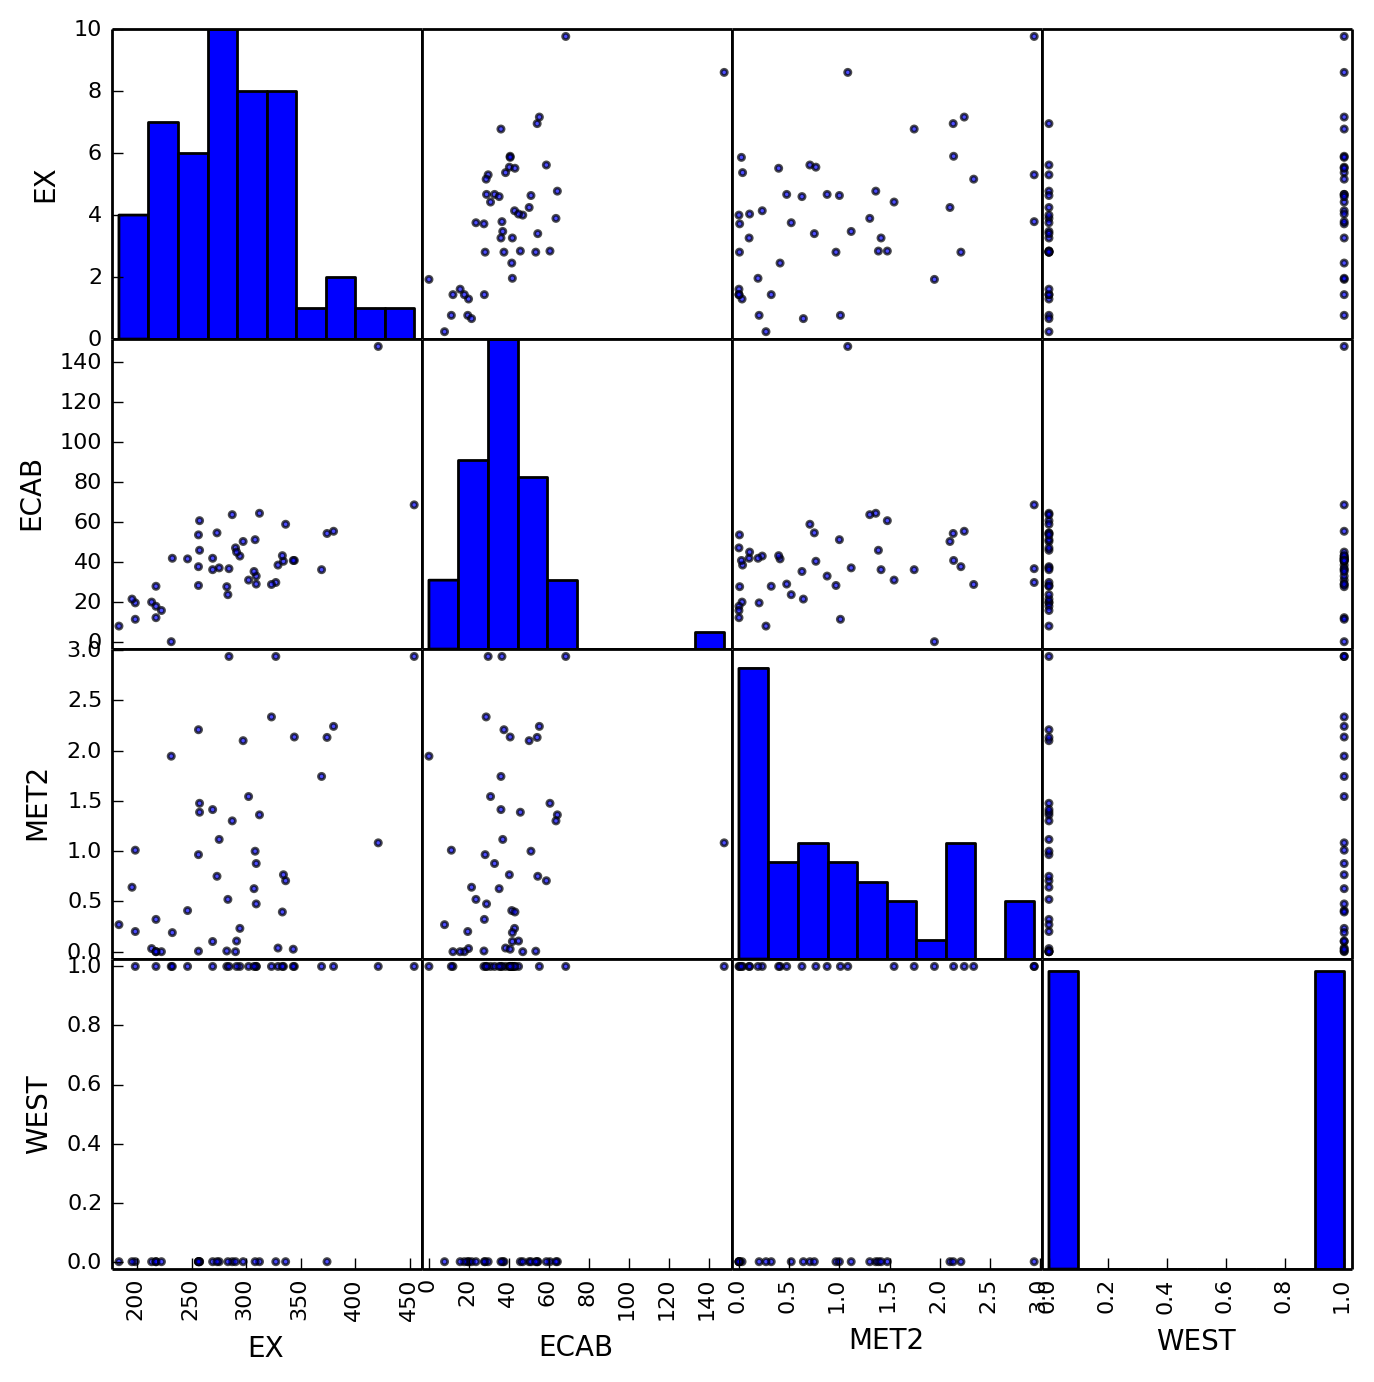
\includegraphics[scale=0.6]{./img/scatter_matrix2.png}
        \caption{Scatter Matrix With Adjusted MET}
        \label{fig:scatter_matrix2}
    \end{figure}
    
    This model is more accurate than our previous model as we've removed all variables that are either collinear or
    don't have enough of an impact on \texttt{EX}. Using only these variables we can much more accurately represent the
    changes in \texttt{EX}.

    \subsection*{Question Five}
    \textbf{Perform a hypothesis test to determine if the predictors removed from the full model from part (3) to create
    the model in (4) should be kept in the model. Provide the hypothesis, perform the test, and state the conclusions
    and p-values. Be sure to provide your answer in terms of the original problem.}\newline

    \begin{itemize}
    \itemsep1pt\parskip0pt\parsep0pt
    \item
      We first establish our Null and Alternate Hypotheses. The subsequent
      test is then performed using the residual sum of squares for each
      model. For these hypotheses, $\beta_j$ is the coefficient of the
      variable that was removed from our model in part 4.
    \end{itemize}

\begin{equation*}
    \begin{cases}
        H_0 \to Y_l \to \text{All $\beta_j$ are equal to 0}\\
        H_\alpha \to Y_k \to \text{At least one $\beta_j$ is not zero}
    \end{cases}
\end{equation*}

\begin{itemize}
\itemsep1pt\parskip0pt\parsep0pt
\item
  We can now perform the test necessary, but we first need our test statistic, $f$, which has $F$ distribution. This is
  found by the following equation.
\end{itemize}

\begin{equation}
    \frac{\left( \text{SSE}_l - \text{SSE}_k \right) / (k - l)}
    {\text{SSE}_k / \left[ n - (k + 1) \right]}
\end{equation}

    \begin{Verbatim}[commandchars=\\\{\}]
\PY{n}{k} \PY{o}{=} \PY{l+m+mi}{7}   \PY{c}{\PYZsh{} Establish constants}
\PY{n}{l} \PY{o}{=} \PY{l+m+mi}{3}
\PY{n}{n} \PY{o}{=} \PY{l+m+mi}{48}
\end{Verbatim}

    We use \texttt{R} to determine our $\sum {\left( y_i - \hat{y_i} \right)}^2$, or our residual sum of squares for
    each model.

    \begin{Verbatim}[commandchars=\\\{\}]
\PY{o}{\PYZpc{}\PYZpc{}}\PY{k}{R} \PY{o}{\PYZhy{}}\PY{n}{i} \PY{n}{data} \PY{o}{\PYZhy{}}\PY{n}{o} \PY{n}{sse}
\PY{n}{fit\PYZus{}full} \PY{o}{\PYZlt{}}\PY{o}{\PYZhy{}} \PY{n}{lm}\PY{p}{(}\PY{n}{EX} \PY{o}{\PYZti{}} \PY{n}{ECAB} \PY{o}{+} \PY{n}{MET} \PY{o}{+} \PY{n}{MET2} \PY{o}{+} \PY{n}{GROW}
             \PY{o}{+} \PY{n}{YOUNG} \PY{o}{+} \PY{n}{OLD} \PY{o}{+} \PY{n}{WEST}\PY{p}{,} \PY{n}{data}\PY{o}{=}\PY{n}{data}\PY{p}{)}
\PY{n}{fit\PYZus{}small} \PY{o}{\PYZlt{}}\PY{o}{\PYZhy{}} \PY{n}{lm}\PY{p}{(}\PY{n}{EX} \PY{o}{\PYZti{}} \PY{n}{ECAB} \PY{o}{+} \PY{n}{MET2} \PY{o}{+} \PY{n}{WEST}\PY{p}{,} \PY{n}{data}\PY{o}{=}\PY{n}{data}\PY{p}{)}
\PY{n}{sse} \PY{o}{\PYZlt{}}\PY{o}{\PYZhy{}} \PY{n}{c}\PY{p}{(}\PY{n}{deviance}\PY{p}{(}\PY{n}{fit\PYZus{}full}\PY{p}{)}\PY{p}{,} \PY{n}{deviance}\PY{p}{(}\PY{n}{fit\PYZus{}small}\PY{p}{)}\PY{p}{)}
\end{Verbatim}

    Finally we implement our equation.

\begin{Verbatim}[commandchars=\\\{\}]
\PY{n}{f} \PY{o}{=} \PY{p}{(}\PY{p}{(}\PY{p}{(}\PY{n}{sse}\PY{p}{[}\PY{l+m+mi}{1}\PY{p}{]} \PY{o}{\PYZhy{}} \PY{n}{sse}\PY{p}{[}\PY{l+m+mi}{0}\PY{p}{]}\PY{p}{)} \PY{o}{/} \PY{p}{(}\PY{n}{k} \PY{o}{\PYZhy{}} \PY{n}{l}\PY{p}{)}\PY{p}{)} \PY{o}{/}
              \PY{p}{(}\PY{n}{sse}\PY{p}{[}\PY{l+m+mi}{0}\PY{p}{]} \PY{o}{/} \PY{p}{(}\PY{n}{n} \PY{o}{\PYZhy{}} \PY{p}{(}\PY{n}{k} \PY{o}{+} \PY{l+m+mi}{1}\PY{p}{)}\PY{p}{)}\PY{p}{)}\PY{p}{)}
Test Statistic: 0.909796312571
\end{Verbatim}

    \begin{itemize}
\itemsep1pt\parskip0pt\parsep0pt
\item
  We can now compare our value of $f$ with $F_{\alpha, k - l, n - (k + 1)}$. We reject $H_0$ if $f$ is greater than or
  equal to our $F$ distribution using a confidence level of $\alpha = 0.05$.
\end{itemize}

\begin{Verbatim}[commandchars=\\\{\}]
\PY{n}{F} \PY{o}{=} \PY{n}{stats}\PY{o}{.}\PY{n}{f}\PY{o}{.}\PY{n}{ppf}\PY{p}{(}\PY{l+m+mf}{0.95}\PY{p}{,} \PY{n}{k} \PY{o}{\PYZhy{}} \PY{n}{l}\PY{p}{,} \PY{n}{n} \PY{o}{\PYZhy{}} \PY{p}{(}\PY{n}{k} \PY{o}{+} \PY{l+m+mi}{1}\PY{p}{)}\PY{p}{)}
Do we Reject? False
\end{Verbatim}

    \begin{itemize}
\itemsep1pt\parskip0pt\parsep0pt
\item
  Therefore we now know that we should use our purged model, as it better explains the variation in \texttt{EX}. We also
  examine the p-values to make sure that our test statistic is reasonable.
\end{itemize}

    \begin{Verbatim}[commandchars=\\\{\}]
\PY{n}{p} \PY{o}{=} \PY{n}{stats}\PY{o}{.}\PY{n}{f}\PY{o}{.}\PY{n}{cdf}\PY{p}{(}\PY{n}{f}\PY{p}{,} \PY{n}{k} \PY{o}{\PYZhy{}} \PY{n}{l}\PY{p}{,} \PY{n}{n} \PY{o}{\PYZhy{}} \PY{p}{(}\PY{n}{k} \PY{o}{+} \PY{l+m+mi}{1}\PY{p}{)}\PY{p}{)}
P-Value:  0.532449100876
\end{Verbatim}

    Since our p-value is above $0.1$ there is no presumption against the
null hypothesis, and our calculated test stastic is reasonable.

    \subsection*{Question Six}
    \textbf{Software-performed model selection: Use a built-in model selection routine on the full model from part (3).
    You may pick whatever routine you would like, but you must provide a short description of the routine and how it
    performs model selection. Write out the estimated regression model that the routine selects as best. Does this
    model match the model from part (4)? If not, do you think this model is better or worse? Why? Notice that this
    portion is worth the most points in this section, so be very thorough with your answer.}\newline


    We will use \texttt{R} for this part, as the libraries available to \texttt{python} are a little less developed. The
    tool in question is called \texttt{stepAIC} from the \texttt{MASS} package which iterates through our data,
    eliminating collinear variables as it goes.

    In order to find the best combination of variables we need to maximize $R^2$, but minimize the amount of variables.
    We are primarily interested in three parameters:

\begin{enumerate}
\def\labelenumi{\arabic{enumi}.}
\itemsep1pt\parskip0pt\parsep0pt
\item
  $R^2_k \to$ The coefficient of multiple determination explains how
  much variation in \texttt{EX} is explained by the current model with
  $k$ variables.
\item
  $\text{MSE}_k \to \frac{\text{SSE}_k}{n - k - 1} \to$ The mean squared
  error for the given model, which we wish to minimize. This
  consideration is considered equivalent to the consideration of the
  adjusted $R^2_k$.
\item
  $C_k \to \frac{\text{SSE}_k}{s^2} + 2(k + 1) - n \to$ This somewhat
  abstract criteria must be minimized.
\end{enumerate}

There are two ways two select the proper variables, forward and backward
selection.

\begin{itemize}
\itemsep1pt\parskip0pt\parsep0pt
\item
  Forward Selection

  \begin{enumerate}
  \def\labelenumi{\arabic{enumi}.}
  \itemsep1pt\parskip0pt\parsep0pt
  \item
    Start with all variables, eliminate one at a time
  \end{enumerate}
\item
  Backward Selection

  \begin{enumerate}
  \def\labelenumi{\arabic{enumi}.}
  \itemsep1pt\parskip0pt\parsep0pt
  \item
    Start with no variables, add one by one
  \end{enumerate}
\end{itemize}

    \begin{Verbatim}[commandchars=\\\{\}]
\PY{o}{\PYZpc{}\PYZpc{}}\PY{k}{R} \PY{o}{\PYZhy{}}\PY{n}{i} \PY{n}{data}
\PY{n}{library}\PY{p}{(}\PY{l+s}{\PYZsq{}}\PY{l+s}{MASS}\PY{l+s}{\PYZsq{}}\PY{p}{)}
\PY{n}{df} \PY{o}{\PYZlt{}}\PY{o}{\PYZhy{}} \PY{n}{data}\PY{o}{.}\PY{n}{frame}\PY{p}{(}\PY{n}{ex}\PY{o}{=}\PY{n}{data}\PY{p}{[}\PY{p}{[}\PY{l+m+mi}{1}\PY{p}{]}\PY{p}{]}\PY{p}{,} \PY{n}{ecab}\PY{o}{=}\PY{n}{data}\PY{p}{[}\PY{p}{[}\PY{l+m+mi}{2}\PY{p}{]}\PY{p}{]}\PY{p}{,} 
               \PY{n}{met}\PY{o}{=}\PY{n}{data}\PY{p}{[}\PY{p}{[}\PY{l+m+mi}{3}\PY{p}{]}\PY{p}{]}\PY{p}{,} \PY{n}{grow}\PY{o}{=}\PY{n}{data}\PY{p}{[}\PY{p}{[}\PY{l+m+mi}{4}\PY{p}{]}\PY{p}{]}\PY{p}{,} 
               \PY{n}{young}\PY{o}{=}\PY{n}{data}\PY{p}{[}\PY{p}{[}\PY{l+m+mi}{5}\PY{p}{]}\PY{p}{]}\PY{p}{,} \PY{n}{old}\PY{o}{=}\PY{n}{data}\PY{p}{[}\PY{p}{[}\PY{l+m+mi}{6}\PY{p}{]}\PY{p}{]}\PY{p}{,}
               \PY{n}{west}\PY{o}{=}\PY{n}{data}\PY{p}{[}\PY{p}{[}\PY{l+m+mi}{7}\PY{p}{]}\PY{p}{]}\PY{p}{,} \PY{n}{met2}\PY{o}{=}\PY{n}{data}\PY{p}{[}\PY{p}{[}\PY{l+m+mi}{10}\PY{p}{]}\PY{p}{]}\PY{p}{)}
\PY{n}{fit} \PY{o}{\PYZlt{}}\PY{o}{\PYZhy{}} \PY{n}{lm}\PY{p}{(}\PY{n}{ex}\PY{o}{\PYZti{}}\PY{n}{ecab} \PY{o}{+} \PY{n}{met} \PY{o}{+} \PY{n}{grow} \PY{o}{+} \PY{n}{young} \PY{o}{+} \PY{n}{old} \PY{o}{+} \PY{n}{west} \PY{o}{+} \PY{n}{met2}\PY{p}{,} \PY{n}{data}\PY{o}{=}\PY{n}{df}\PY{p}{)}
\PY{n}{step} \PY{o}{\PYZlt{}}\PY{o}{\PYZhy{}} \PY{n}{stepAIC}\PY{p}{(}\PY{n}{fit}\PY{p}{,} \PY{n}{direction}\PY{o}{=}\PY{l+s}{\PYZsq{}}\PY{l+s}{both}\PY{l+s}{\PYZsq{}}\PY{p}{)}
\PY{n}{step}\PY{err}{\PYZdl{}}\PY{n}{anova}
\end{Verbatim}

    
    \begin{verbatim}
Initial Model:
ex ~ ecab + met + grow + young + old + west + met2

Final Model:
ex ~ ecab + grow + west + met2

     Step Df    Deviance Resid. Df Resid. Dev      AIC
1                               40   50155.02 349.6803
2 - young  1    9.514664        41   50164.54 347.6894
3   - met  1  857.107838        42   51021.64 346.5026
4   - old  1 1121.551966        43   52143.19 345.5463

    \end{verbatim}

    
    This yields a final model of

\begin{equation}
    \text{EX} = \hat{\beta}_0 +
                \hat{\beta}_1 \text{ECAB} +
                \hat{\beta}_2 \text{GROW} +
                \hat{\beta}_3 \text{WEST} +
                \hat{\beta}_4 \text{MET2}
\end{equation}

Which is better than our previous models as it examines all combinations
of the variables.

\subsection*{Question Seven}
    \textbf{Between the models created in part (4) and part (6), pick your favorite. Check the assumptions of this
    model. Does it seem that this model has satisfied these assumptions?}\newline

    I really like the model I created in part (6), which I'll restate here
just because it's my favorite.

\begin{equation}
    \text{EX} = \hat{\beta}_0 +
                \hat{\beta}_1 \text{ECAB} +
                \hat{\beta}_2 \text{GROW} +
                \hat{\beta}_3 \text{WEST} +
                \hat{\beta}_4 \text{MET2}
\end{equation}

Which looks like the following.

    \begin{Verbatim}[commandchars=\\\{\}]
 \PY{n}{purged\PYZus{}multi\PYZus{}regression} \PY{o}{=} \PY{n}{sm}\PY{o}{.}\PY{n}{ols}\PY{p}{(}\PY{n}{formula}\PY{o}{=}\PY{l+s}{\PYZsq{}\PYZsq{}\PYZsq{}}\PY{l+s}{EX \PYZti{} ECAB + GROW + MET2 + WEST}\PY{l+s}{\PYZsq{}\PYZsq{}\PYZsq{}}\PY{p}{,} \PY{n}{data}\PY{o}{=}\PY{n}{data}\PY{p}{)}\PY{o}{.}\PY{n}{fit}\PY{p}{(}\PY{p}{)}
          \PY{n}{purged\PYZus{}multi\PYZus{}regression}\PY{o}{.}\PY{n}{summary}\PY{p}{(}\PY{p}{)}
\end{Verbatim}

            \begin{Verbatim}[commandchars=\\\{\}]
          """
                                      OLS Regression Results                            
          ==============================================================================
          Dep. Variable:                     EX   R-squared:                       0.679
          Model:                            OLS   Adj. R-squared:                  0.649
          Method:                 Least Squares   F-statistic:                     22.75
          Date:                Wed, 07 May 2014   Prob (F-statistic):           3.81e-10
          Time:                        01:21:43   Log-Likelihood:                -235.88
          No. Observations:                  48   AIC:                             481.8
          Df Residuals:                      43   BIC:                             491.1
          Df Model:                           4                                         
          Covariance Type:            nonrobust                                         
          ==============================================================================
                           coef    std err          t      P>|t|      [95.0\% Conf. Int.]
          ------------------------------------------------------------------------------
          Intercept    183.4190     11.969     15.325      0.000       159.282   207.556
          ECAB           1.3404      0.264      5.087      0.000         0.809     1.872
          GROW           0.4452      0.306      1.457      0.152        -0.171     1.061
          MET2          23.4206      5.845      4.007      0.000        11.633    35.209
          WEST          38.4123     10.094      3.806      0.000        18.057    58.768
          ==============================================================================
          Omnibus:                        0.407   Durbin-Watson:                   2.735
          Prob(Omnibus):                  0.816   Jarque-Bera (JB):                0.556
          Skew:                           0.014   Prob(JB):                        0.757
          Kurtosis:                       2.473   Cond. No.                         132.
          ==============================================================================
          
          Warnings:
          [1] Standard Errors assume that the covariance matrix of the errors is correctly specified.
          """
\end{Verbatim}
        
    There are four assumptions of the model which we can examine.

\begin{enumerate}
\def\labelenumi{\arabic{enumi}.}
\itemsep1pt\parskip0pt\parsep0pt
\item
  Linearity of the relationship between dependent and independent
  variables
\item
  Independence of the errors (no serial correlation)
\item
  Homoscedasticity (constant variance) of the errors

  \begin{enumerate}
  \def\labelenumii{\arabic{enumii}.}
  \itemsep1pt\parskip0pt\parsep0pt
  \item
    versus time
  \item
    versus the predictions (or versus any independent variable)
  \end{enumerate}
\item
  Normality of the error distribution.
\end{enumerate}

We will examine each assumption individually using diagnostic plots.

\textbf{Linearity}

For linearity we will plot the
\texttt{Observed Values\textasciitilde{}Predicted Values} and the
\texttt{Residuals\textasciitilde{}Predicted Values}. We first use
\texttt{R} to determine the residuals for our model, as well as our
fitted values, $\hat{y}$.

    \begin{Verbatim}[commandchars=\\\{\}]
 \PY{o}{\PYZpc{}}\PY{k}{R} \PY{o}{\PYZhy{}}\PY{n}{i} \PY{n}{data} \PY{n}{fit} \PY{o}{\PYZlt{}}\PY{o}{\PYZhy{}} \PY{n}{lm}\PY{p}{(}\PY{n}{EX} \PY{o}{\PYZti{}} \PY{n}{ECAB} \PY{o}{+} \PY{n}{GROW} \PY{o}{+} \PY{n}{WEST} \PY{o}{+} \PY{n}{MET2}\PY{p}{,} \PY{n}{data}\PY{o}{=}\PY{n}{data}\PY{p}{)}
          \PY{o}{\PYZpc{}}\PY{k}{R} \PY{o}{\PYZhy{}}\PY{n}{o} \PY{n}{r}\PY{p}{,}\PY{n}{yh} \PY{n}{r} \PY{o}{\PYZlt{}}\PY{o}{\PYZhy{}} \PY{n}{residuals}\PY{p}{(}\PY{n}{fit}\PY{p}{)}\PY{p}{;} \PY{n}{yh} \PY{o}{\PYZlt{}}\PY{o}{\PYZhy{}} \PY{n}{fitted}\PY{p}{(}\PY{n}{fit}\PY{p}{)}
\end{Verbatim}

            \begin{Verbatim}[commandchars=\\\{\}]
 array([ 246.76589624,  265.58001954,  293.53320353,  304.27903757,
                  285.84578381,  312.66313097,  311.60135975,  310.44023448,
                  280.64162961,  296.3931407 ,  278.63149143,  220.431476  ,
                  285.06956775,  283.60906205,  263.26293335,  305.9126729 ,
                  252.91690939,  224.7764192 ,  214.2564556 ,  210.75435475,
                  232.5036399 ,  205.91479801,  210.74112334,  261.47566014,
                  241.04280851,  267.60454393,  280.42857451,  286.98677517,
                  286.52948096,  312.20562753,  301.31370148,  283.12186639,
                  290.46107077,  324.61519378,  257.72998807,  261.70705142,
                  297.63520969,  289.10405759,  319.42226914,  299.60756465,
                  345.46831432,  388.40416046,  340.29536166,  296.34157683,
                  297.57903212,  283.81829211,  479.66794847,  369.90953046])
\end{Verbatim}
        
    We can now use diagnostic plots on these determined values.

    \begin{Verbatim}[commandchars=\\\{\}]
 \PY{n}{fig}\PY{p}{,} \PY{n}{ax} \PY{o}{=} \PY{n}{plt}\PY{o}{.}\PY{n}{subplots}\PY{p}{(}\PY{l+m+mi}{2}\PY{p}{,} \PY{l+m+mi}{1}\PY{p}{)}
          \PY{n}{ax}\PY{p}{[}\PY{l+m+mi}{0}\PY{p}{]}\PY{o}{.}\PY{n}{scatter}\PY{p}{(}\PY{n}{data}\PY{p}{[}\PY{l+s}{\PYZsq{}}\PY{l+s}{EX}\PY{l+s}{\PYZsq{}}\PY{p}{]}\PY{p}{,} \PY{n}{yh}\PY{p}{,} \PY{n}{label}\PY{o}{=}\PY{l+s}{r\PYZsq{}}\PY{l+s}{EX\PYZti{}\PYZdl{}}\PY{l+s}{\PYZbs{}}\PY{l+s}{hat\PYZob{}y\PYZcb{}\PYZdl{}}\PY{l+s}{\PYZsq{}}\PY{p}{)}
          \PY{n}{ax}\PY{p}{[}\PY{l+m+mi}{0}\PY{p}{]}\PY{o}{.}\PY{n}{plot}\PY{p}{(}\PY{n}{np}\PY{o}{.}\PY{n}{arange}\PY{p}{(}\PY{l+m+mi}{100}\PY{p}{,} \PY{l+m+mi}{600}\PY{p}{)}\PY{p}{,} \PY{n}{np}\PY{o}{.}\PY{n}{arange}\PY{p}{(}\PY{l+m+mi}{100}\PY{p}{,} \PY{l+m+mi}{600}\PY{p}{)}\PY{p}{,} \PY{l+s}{\PYZsq{}}\PY{l+s}{k\PYZhy{}\PYZhy{}}\PY{l+s}{\PYZsq{}}\PY{p}{,} \PY{n}{label}\PY{o}{=}\PY{l+s}{r\PYZsq{}}\PY{l+s}{\PYZdl{}y=x\PYZdl{}}\PY{l+s}{\PYZsq{}}\PY{p}{)}
          \PY{n}{ax}\PY{p}{[}\PY{l+m+mi}{1}\PY{p}{]}\PY{o}{.}\PY{n}{scatter}\PY{p}{(}\PY{n}{yh}\PY{p}{,} \PY{n}{r}\PY{p}{,} \PY{n}{label}\PY{o}{=}\PY{l+s}{r\PYZsq{}}\PY{l+s}{\PYZdl{}}\PY{l+s}{\PYZbs{}}\PY{l+s}{hat\PYZob{}y\PYZcb{}\PYZdl{}\PYZti{}Residuals}\PY{l+s}{\PYZsq{}}\PY{p}{)}
          \PY{n}{ax}\PY{p}{[}\PY{l+m+mi}{1}\PY{p}{]}\PY{o}{.}\PY{n}{plot}\PY{p}{(}\PY{n}{np}\PY{o}{.}\PY{n}{arange}\PY{p}{(}\PY{l+m+mi}{100}\PY{p}{,} \PY{l+m+mi}{600}\PY{p}{)}\PY{p}{,} \PY{n}{np}\PY{o}{.}\PY{n}{zeros}\PY{p}{(}\PY{l+m+mi}{500}\PY{p}{)}\PY{p}{,} \PY{l+s}{\PYZsq{}}\PY{l+s}{k\PYZhy{}\PYZhy{}}\PY{l+s}{\PYZsq{}}\PY{p}{,} \PY{n}{label}\PY{o}{=}\PY{l+s}{r\PYZsq{}}\PY{l+s}{\PYZdl{}y=0\PYZdl{}}\PY{l+s}{\PYZsq{}}\PY{p}{)}
          \PY{n}{ax}\PY{p}{[}\PY{l+m+mi}{0}\PY{p}{]}\PY{o}{.}\PY{n}{set\PYZus{}xlabel}\PY{p}{(}\PY{l+s}{\PYZsq{}}\PY{l+s}{Observed Values}\PY{l+s}{\PYZsq{}}\PY{p}{)}
          \PY{n}{ax}\PY{p}{[}\PY{l+m+mi}{0}\PY{p}{]}\PY{o}{.}\PY{n}{set\PYZus{}ylabel}\PY{p}{(}\PY{l+s}{\PYZsq{}}\PY{l+s}{Predicted Values}\PY{l+s}{\PYZsq{}}\PY{p}{)}
          \PY{n}{ax}\PY{p}{[}\PY{l+m+mi}{1}\PY{p}{]}\PY{o}{.}\PY{n}{set\PYZus{}ylabel}\PY{p}{(}\PY{l+s}{\PYZsq{}}\PY{l+s}{Residuals}\PY{l+s}{\PYZsq{}}\PY{p}{)}
          \PY{n}{ax}\PY{p}{[}\PY{l+m+mi}{1}\PY{p}{]}\PY{o}{.}\PY{n}{set\PYZus{}xlabel}\PY{p}{(}\PY{l+s}{\PYZsq{}}\PY{l+s}{Predicted Values}\PY{l+s}{\PYZsq{}}\PY{p}{)}
          \PY{n}{ax}\PY{p}{[}\PY{l+m+mi}{0}\PY{p}{]}\PY{o}{.}\PY{n}{grid}\PY{p}{(}\PY{n+nb+bp}{True}\PY{p}{,} \PY{n}{which}\PY{o}{=}\PY{l+s}{\PYZsq{}}\PY{l+s}{both}\PY{l+s}{\PYZsq{}}\PY{p}{)}
          \PY{n}{ax}\PY{p}{[}\PY{l+m+mi}{1}\PY{p}{]}\PY{o}{.}\PY{n}{grid}\PY{p}{(}\PY{n+nb+bp}{True}\PY{p}{,} \PY{n}{which}\PY{o}{=}\PY{l+s}{\PYZsq{}}\PY{l+s}{both}\PY{l+s}{\PYZsq{}}\PY{p}{)}
          \PY{n}{handles}\PY{p}{,} \PY{n}{labels} \PY{o}{=} \PY{n}{ax}\PY{p}{[}\PY{l+m+mi}{0}\PY{p}{]}\PY{o}{.}\PY{n}{get\PYZus{}legend\PYZus{}handles\PYZus{}labels}\PY{p}{(}\PY{p}{)}
          \PY{n}{ax}\PY{p}{[}\PY{l+m+mi}{0}\PY{p}{]}\PY{o}{.}\PY{n}{legend}\PY{p}{(}\PY{n}{handles}\PY{p}{,} \PY{n}{labels}\PY{p}{)}
          \PY{n}{handles}\PY{p}{,} \PY{n}{labels} \PY{o}{=} \PY{n}{ax}\PY{p}{[}\PY{l+m+mi}{1}\PY{p}{]}\PY{o}{.}\PY{n}{get\PYZus{}legend\PYZus{}handles\PYZus{}labels}\PY{p}{(}\PY{p}{)}
          \PY{n}{ax}\PY{p}{[}\PY{l+m+mi}{1}\PY{p}{]}\PY{o}{.}\PY{n}{legend}\PY{p}{(}\PY{n}{handles}\PY{p}{,} \PY{n}{labels}\PY{p}{)}
          \PY{n}{plt}\PY{o}{.}\PY{n}{show}\PY{p}{(}\PY{p}{)}
\end{Verbatim}

    \begin{center}
    \adjustimage{max size={0.9\linewidth}{0.9\paperheight}}{Takehome_Final_files/Takehome_Final_59_0.png}
    \end{center}
    { \hspace*{\fill} \\}
    
    In our first plot our data follows a diagonal line. This is good as it
show a strong linear relationship between our predictions and our
observations. In the perfect world this would be a direct 1-1
correspondence, as the line $y=x$ is ideal.

In the second plot our values are for the most part centered around a
horizontal line. Again, this is good as it shows that our residuals are
static and normally distributed.

\textbf{Independence}

For independence we will examine the scatter matrix and examine our
variables.

    \begin{Verbatim}[commandchars=\\\{\}]
 \PY{n}{sc\PYZus{}matrix} \PY{o}{=} \PY{n}{pp}\PY{o}{.}\PY{n}{scatter\PYZus{}matrix}\PY{p}{(}\PY{n}{data}\PY{p}{[}\PY{p}{[}\PY{l+s}{\PYZsq{}}\PY{l+s}{EX}\PY{l+s}{\PYZsq{}}\PY{p}{,} \PY{l+s}{\PYZsq{}}\PY{l+s}{ECAB}\PY{l+s}{\PYZsq{}}\PY{p}{,} \PY{l+s}{\PYZsq{}}\PY{l+s}{GROW}\PY{l+s}{\PYZsq{}}\PY{p}{,} \PY{l+s}{\PYZsq{}}\PY{l+s}{MET2}\PY{l+s}{\PYZsq{}}\PY{p}{,} \PY{l+s}{\PYZsq{}}\PY{l+s}{WEST}\PY{l+s}{\PYZsq{}}\PY{p}{]}\PY{p}{]}\PY{p}{,}
                                        \PY{n}{alpha}\PY{o}{=}\PY{l+m+mf}{0.7}\PY{p}{)}
\end{Verbatim}

    \begin{center}
    \adjustimage{max size={0.9\linewidth}{0.9\paperheight}}{Takehome_Final_files/Takehome_Final_61_0.png}
    \end{center}
    { \hspace*{\fill} \\}
    
    By examining our scatter matrix we can determine that for the most part
only our dependent and independent variables have a linear relation.
This is good, as it shows we've removed variables that have a linear
relationship between other variables.

\textbf{Homoscedasticity}

We will examine \texttt{Residuals\textasciitilde{}Time} and
\texttt{Residuals\textasciitilde{}Predicted Value}.

    \begin{Verbatim}[commandchars=\\\{\}]
 \PY{n}{fig}\PY{p}{,} \PY{n}{ax} \PY{o}{=} \PY{n}{plt}\PY{o}{.}\PY{n}{subplots}\PY{p}{(}\PY{l+m+mi}{2}\PY{p}{,} \PY{l+m+mi}{1}\PY{p}{)}
          \PY{n}{ax}\PY{p}{[}\PY{l+m+mi}{0}\PY{p}{]}\PY{o}{.}\PY{n}{plot}\PY{p}{(}\PY{n}{np}\PY{o}{.}\PY{n}{arange}\PY{p}{(}\PY{l+m+mi}{0}\PY{p}{,} \PY{l+m+mi}{48}\PY{p}{)}\PY{p}{,} \PY{n}{r}\PY{p}{,} \PY{n}{label}\PY{o}{=}\PY{l+s}{\PYZsq{}}\PY{l+s}{Residuals over Time}\PY{l+s}{\PYZsq{}}\PY{p}{)}
          \PY{n}{ax}\PY{p}{[}\PY{l+m+mi}{0}\PY{p}{]}\PY{o}{.}\PY{n}{plot}\PY{p}{(}\PY{n}{np}\PY{o}{.}\PY{n}{arange}\PY{p}{(}\PY{l+m+mi}{0}\PY{p}{,} \PY{l+m+mi}{49}\PY{p}{)}\PY{p}{,} \PY{n}{np}\PY{o}{.}\PY{n}{zeros}\PY{p}{(}\PY{l+m+mi}{49}\PY{p}{)}\PY{p}{,} \PY{l+s}{\PYZsq{}}\PY{l+s}{k\PYZhy{}\PYZhy{}}\PY{l+s}{\PYZsq{}}\PY{p}{,} \PY{n}{label}\PY{o}{=}\PY{l+s}{r\PYZsq{}}\PY{l+s}{\PYZdl{}y=0\PYZdl{}}\PY{l+s}{\PYZsq{}}\PY{p}{)}
          \PY{n}{ax}\PY{p}{[}\PY{l+m+mi}{1}\PY{p}{]}\PY{o}{.}\PY{n}{scatter}\PY{p}{(}\PY{n}{yh}\PY{p}{,} \PY{n}{r}\PY{p}{,} \PY{n}{label}\PY{o}{=}\PY{l+s}{r\PYZsq{}}\PY{l+s}{\PYZdl{}}\PY{l+s}{\PYZbs{}}\PY{l+s}{hat\PYZob{}y\PYZcb{}\PYZdl{}\PYZti{}Residuals}\PY{l+s}{\PYZsq{}}\PY{p}{)}
          \PY{n}{ax}\PY{p}{[}\PY{l+m+mi}{1}\PY{p}{]}\PY{o}{.}\PY{n}{plot}\PY{p}{(}\PY{n}{np}\PY{o}{.}\PY{n}{arange}\PY{p}{(}\PY{l+m+mi}{100}\PY{p}{,} \PY{l+m+mi}{600}\PY{p}{)}\PY{p}{,} \PY{n}{np}\PY{o}{.}\PY{n}{zeros}\PY{p}{(}\PY{l+m+mi}{500}\PY{p}{)}\PY{p}{,} \PY{l+s}{\PYZsq{}}\PY{l+s}{k\PYZhy{}\PYZhy{}}\PY{l+s}{\PYZsq{}}\PY{p}{,} \PY{n}{label}\PY{o}{=}\PY{l+s}{r\PYZsq{}}\PY{l+s}{\PYZdl{}y=0\PYZdl{}}\PY{l+s}{\PYZsq{}}\PY{p}{)}
          \PY{n}{ax}\PY{p}{[}\PY{l+m+mi}{0}\PY{p}{]}\PY{o}{.}\PY{n}{set\PYZus{}xlabel}\PY{p}{(}\PY{l+s}{\PYZsq{}}\PY{l+s}{\PYZdq{}}\PY{l+s}{Time}\PY{l+s}{\PYZdq{}}\PY{l+s}{\PYZsq{}}\PY{p}{)}
          \PY{n}{ax}\PY{p}{[}\PY{l+m+mi}{0}\PY{p}{]}\PY{o}{.}\PY{n}{set\PYZus{}ylabel}\PY{p}{(}\PY{l+s}{\PYZsq{}}\PY{l+s}{Residuals}\PY{l+s}{\PYZsq{}}\PY{p}{)}
          \PY{n}{ax}\PY{p}{[}\PY{l+m+mi}{1}\PY{p}{]}\PY{o}{.}\PY{n}{set\PYZus{}ylabel}\PY{p}{(}\PY{l+s}{\PYZsq{}}\PY{l+s}{Residuals}\PY{l+s}{\PYZsq{}}\PY{p}{)}
          \PY{n}{ax}\PY{p}{[}\PY{l+m+mi}{1}\PY{p}{]}\PY{o}{.}\PY{n}{set\PYZus{}xlabel}\PY{p}{(}\PY{l+s}{\PYZsq{}}\PY{l+s}{Predicted Values}\PY{l+s}{\PYZsq{}}\PY{p}{)}
          \PY{n}{ax}\PY{p}{[}\PY{l+m+mi}{0}\PY{p}{]}\PY{o}{.}\PY{n}{grid}\PY{p}{(}\PY{n+nb+bp}{True}\PY{p}{,} \PY{n}{which}\PY{o}{=}\PY{l+s}{\PYZsq{}}\PY{l+s}{both}\PY{l+s}{\PYZsq{}}\PY{p}{)}
          \PY{n}{ax}\PY{p}{[}\PY{l+m+mi}{1}\PY{p}{]}\PY{o}{.}\PY{n}{grid}\PY{p}{(}\PY{n+nb+bp}{True}\PY{p}{,} \PY{n}{which}\PY{o}{=}\PY{l+s}{\PYZsq{}}\PY{l+s}{both}\PY{l+s}{\PYZsq{}}\PY{p}{)}
          \PY{n}{ax}\PY{p}{[}\PY{l+m+mi}{0}\PY{p}{]}\PY{o}{.}\PY{n}{set\PYZus{}ylim}\PY{p}{(}\PY{p}{(}\PY{o}{\PYZhy{}}\PY{l+m+mi}{120}\PY{p}{,} \PY{l+m+mi}{120}\PY{p}{)}\PY{p}{)}
          \PY{n}{handles}\PY{p}{,} \PY{n}{labels} \PY{o}{=} \PY{n}{ax}\PY{p}{[}\PY{l+m+mi}{0}\PY{p}{]}\PY{o}{.}\PY{n}{get\PYZus{}legend\PYZus{}handles\PYZus{}labels}\PY{p}{(}\PY{p}{)}
          \PY{n}{ax}\PY{p}{[}\PY{l+m+mi}{0}\PY{p}{]}\PY{o}{.}\PY{n}{legend}\PY{p}{(}\PY{n}{handles}\PY{p}{,} \PY{n}{labels}\PY{p}{)}
          \PY{n}{handles}\PY{p}{,} \PY{n}{labels} \PY{o}{=} \PY{n}{ax}\PY{p}{[}\PY{l+m+mi}{1}\PY{p}{]}\PY{o}{.}\PY{n}{get\PYZus{}legend\PYZus{}handles\PYZus{}labels}\PY{p}{(}\PY{p}{)}
          \PY{n}{ax}\PY{p}{[}\PY{l+m+mi}{1}\PY{p}{]}\PY{o}{.}\PY{n}{legend}\PY{p}{(}\PY{n}{handles}\PY{p}{,} \PY{n}{labels}\PY{p}{)}
          \PY{n}{plt}\PY{o}{.}\PY{n}{show}\PY{p}{(}\PY{p}{)}
\end{Verbatim}

    \begin{center}
    \adjustimage{max size={0.9\linewidth}{0.9\paperheight}}{Takehome_Final_files/Takehome_Final_63_0.png}
    \end{center}
    { \hspace*{\fill} \\}
    
    Our first plot is good as it shows a steady range of residuals that
aren't growing larger or smaller. Our second plot on the other hand
shows our residuals growing larger (more spread out) as our predicted
values increase. This is bad.

\textbf{Normality}

We will create a normal probability plot of the residuals by first
standardizing and then plotting.

    \begin{Verbatim}[commandchars=\\\{\}]
 \PY{n}{fig}\PY{p}{,} \PY{n}{ax} \PY{o}{=} \PY{n}{plt}\PY{o}{.}\PY{n}{subplots}\PY{p}{(}\PY{p}{)}
          \PY{n}{std\PYZus{}res} \PY{o}{=} \PY{p}{(}\PY{n}{r} \PY{o}{\PYZhy{}} \PY{n}{mean}\PY{p}{(}\PY{n}{r}\PY{p}{)}\PY{p}{)} \PY{o}{/} \PY{n}{np}\PY{o}{.}\PY{n}{std}\PY{p}{(}\PY{n}{r}\PY{p}{)}
          \PY{n}{ax}\PY{o}{.}\PY{n}{hist}\PY{p}{(}\PY{n}{std\PYZus{}res}\PY{p}{,} \PY{n}{bins}\PY{o}{=}\PY{l+m+mi}{15}\PY{p}{,} \PY{n}{label}\PY{o}{=}\PY{l+s}{\PYZsq{}}\PY{l+s}{Standardized Residuals}\PY{l+s}{\PYZsq{}}\PY{p}{)}
          \PY{n}{x} \PY{o}{=} \PY{n}{np}\PY{o}{.}\PY{n}{arange}\PY{p}{(}\PY{o}{\PYZhy{}}\PY{l+m+mi}{2}\PY{p}{,} \PY{l+m+mi}{2}\PY{p}{,} \PY{l+m+mf}{0.01}\PY{p}{)}
          \PY{n}{normal} \PY{o}{=} \PY{k}{lambda} \PY{n}{x}\PY{p}{:} \PY{n}{stats}\PY{o}{.}\PY{n}{norm}\PY{o}{.}\PY{n}{pdf}\PY{p}{(}\PY{n}{x}\PY{p}{)}
          \PY{n}{ax}\PY{o}{.}\PY{n}{plot}\PY{p}{(}\PY{n}{x}\PY{p}{,} \PY{l+m+mi}{15} \PY{o}{*} \PY{n}{normal}\PY{p}{(}\PY{n}{x}\PY{p}{)}\PY{p}{,} \PY{l+s}{\PYZsq{}}\PY{l+s}{r\PYZhy{}}\PY{l+s}{\PYZsq{}}\PY{p}{,} \PY{n}{linewidth}\PY{o}{=}\PY{l+m+mi}{3}\PY{p}{,} \PY{n}{label}\PY{o}{=}\PY{l+s}{\PYZsq{}}\PY{l+s}{Normal Distribution Curve}\PY{l+s}{\PYZsq{}}\PY{p}{)}
          \PY{n}{handles}\PY{p}{,} \PY{n}{labels} \PY{o}{=} \PY{n}{ax}\PY{o}{.}\PY{n}{get\PYZus{}legend\PYZus{}handles\PYZus{}labels}\PY{p}{(}\PY{p}{)}
          \PY{n}{ax}\PY{o}{.}\PY{n}{legend}\PY{p}{(}\PY{n}{handles}\PY{p}{,} \PY{n}{labels}\PY{p}{)}
          \PY{n}{plt}\PY{o}{.}\PY{n}{show}\PY{p}{(}\PY{p}{)}
\end{Verbatim}

    \begin{center}
    \adjustimage{max size={0.9\linewidth}{0.9\paperheight}}{Takehome_Final_files/Takehome_Final_65_0.png}
    \end{center}
    { \hspace*{\fill} \\}
    
    We note that we only have 48 datapoints, and as a result our data does
not look very normal. That being said, for only having 48 datapoints we
are lucky to have a distribution that is as normally distributed as this
one is.



\subsection*{Question n}
    Write out the estimate of your favorite model, and interpret all the parameters. Be sure to provide
    interpretations in terms of the original problem, including the original scale of the dependent and independent
    variables.\newline

\subsection*{Question n}
    Using your favorite model, are there any outlying observations? You can use an automated routine to find these if
    they exist. If you do find one or more outliers, re-run your favorite model without it/them. What do you notice? Do
    you think it is okay to remove this observation?\newline

\section*{Part Two}

As we discussed in class, the multiple linear regression model:

\begin{equation*}
    \begin{aligned}
        Y_i = \beta_0 + \beta_1 x_{i,1} + \beta_2 x_{i,2} + \cdots \beta_p x_{i,p} + \epsilon_i \qquad i = 1, \ldots, n
    \end{aligned}
\end{equation*}

is commonly expressed in an alternative way:

\begin{equation}\label{eq:lin-reg-mod}
    \begin{aligned}
        &Y& &=& &\mathbf{X}& &\beta& &+& &\epsilon&\\
        &\begin{pmatrix}
            Y_1\\
            Y_2\\
            \vdots\\
            Y_n
        \end{pmatrix}_{n \times 1}&
        &=&
        &\begin{pmatrix}
            1 & x_{1,1} & x_{1,2} & \cdots & x_{1,p}\\
            1 & x_{2,1} & x_{2,2} & \cdots & x_{2,p}\\
            \vdots & \vdots & \vdots & \ddots & \vdots\\
            1 & x_{n,1} & x_{n,2} & \cdots & x_{n,p}\\
        \end{pmatrix}_{n \times p}&
        &\begin{pmatrix}
            \beta_0\\
            \beta_1\\
            \vdots\\
            \beta_p\\
        \end{pmatrix}_{p \times 1}&
        &+&
        &\begin{pmatrix}
            \epsilon_1\\
            \epsilon_2\\
            \vdots\\
            \epsilon_n\\
        \end{pmatrix}_{n \times 1}&
    \end{aligned}
\end{equation}

In this notation, $Y$ is a vector containing the response values for all $n$ observations. The matrix $X$ is called the
``design matrix,'' with the $i$th row containing the $p$ independent variables for the $i$th observation, and a '1' in
the first column for the intercept. We can obtain estimates of the linear regression parameters by minimizing the least
squares equation, which results in:

\begin{equation*}
    \begin{aligned}
        \hat{\beta} = {\left( X^\prime X \right)}^{-1} X^\prime Y
    \end{aligned}
\end{equation*}

We can also use these vectors and matrices to calculate fitted values, residuals, SSE, MSE, etc.

\begin{easylist}[enumerate]
    @ Write a function that, when given $X$ and $Y$,the parameter estimates and associated values for a linear model are
    calculated. (Hint: Double-check that your function works by comparing the results of your function to the results
    you got in part one)\newline

    Include this function in the main portion of your write-up. Be sure it is well annotated so that I can clearly see
    what is calculated at each step.\newline

    This function should return:

    @@ A table that includes the estimate, standard error, t-statistic, and p-value for each parameter in the
    model.\newline
    @@ The SSE of the model\newline
    @@ The $R^2$ and $R^2_a$ for the model\newline
    @@ The F-statistic for the model\newline

    @ Instead of including MET in the model with a squared term, we can create a categorical variable MET-categ that
    denotes which level MET each state is in by dividing MET up into units of 15:

    \begin{equation*}
        \begin{aligned}
            \text{MET-categ} =
            \begin{cases}
                1 \quad \text{if } \text{MET} < 15\\
                2 \quad \text{if } 15 \le \text{MET} < 30\\
                3 \quad \text{if } 30 \le \text{MET} < 45\\
                4 \quad \text{if } 45 \le \text{MET} < 60\\
                5 \quad \text{if } 60 \le \text{MET} < 75\\
                6 \quad \text{if } 75 \le \text{MET}
            \end{cases}
        \end{aligned}
    \end{equation*}

    Using your favorite model from Part One, remove any MET terms from that model, and add in MET-categ Write out your
    model as in equation~\eqref{eq:lin-reg-mod}, using the actual values in the data set, giving the $\beta$ parameters meaningful names.
    You only need to write out the first and last 5 observations (10 total) from the data.\newline

    @ Use the function you created in step (1) to calculate the estimated regression model. Report all aspects of the
    model that were returned to you by your function: the parameter estimate table, the correlation coefficient values,
    and the F-statistic.\newline

    @ Write down your estimated model. Interpret each parameter in terms of the original units of the problem.\newline

    @ Compare this model to your favorite model from Part One. Do we gain or lose information by converting a continuous
    covariate into a categorical covariate? Which model do you think is best and why? Be thorough in your answer -
    remember that you are reporting to the POTUS!\newline
\end{easylist}

\end{document}
